\newcommand\dif\partial
\newcommand\dd{\mathrm{d}}
\section{Compacité}
\subsection{Caractérisation topologique}
\begin{definition}[Axiome de Borel-Lebesgue]
    Un espace topologique $(X,\mathbb{U})$ est dit compact si :
    \begin{itemize}
        \item $X$ est \underline{séparé}
        \item Pour tout $\mathcal{U}\subset \mathbb{U}$ tel que $\bigcup_{U \in \mathcal{U}}U=X$, il existe $\mathcal{U}_0 \in \mathcal{P}_f(\mathcal{U})$ 
 tel que $\bigcup\limits_{U \in \mathcal{U}_0} U =X$. (De toute couverture de $X$ par des ouverts, on peut extraire une sous couverture finie).
    \end{itemize}
\end{definition}
\begin{remarque}
    \begin{align*}
        \bigcup\limits_{} \mathcal{U}&=\{x\in X\ |\ \exists A\in \mathcal{U},\ x\in A\}\\
                                     &=\bigcup\limits_{A\in \mathcal{U}} A
     \end{align*}
\end{remarque}
\begin{remarque}
    On pouvait considérer les familles d'ouverts. Si $X=\bigcup\limits_{i\in I} U_i$ avec $U_i$ ouvert alors $\exists I_0\subset I,\ I_0 $ fini et tq $\bigcup\limits_{i\in I_0} U_i=X$.
\end{remarque}
\begin{remarque}[Intersection de fermés]
   Soit $(X,\mathbb{U})$ compact. Si $(F_i)_{i\in I}$ est une famille de fermés de $X$ tq $\bigcap\limits_{i\in I} F_i=\emptyset ,$ alors $\exists I_0\subset I,\ I_0$ fini et $\bigcap\limits_{i\in I_0} F_i=\emptyset $.\\
   En particulier, si $(F_n)$ est une suite de fermés emboités non vides alors $\bigcap\limits_{n\in \mathbb{N} } F_n\neq \emptyset .$
\end{remarque}
\begin{lemme}
    Soit $(X,\mathbb{U})$ espace topologique séparé et $F\subset X$ compact. Alors $F$ est fermé.
\end{lemme}
\begin{proof}
    Par contraposée, on suppose $F$ non fermé et on va montrer qu'il n'est pas compact.\\
    Comme $F$ non fermé, il existe $x\in \overline{F}\backslash F.$ Soit $y\in F,$ $V_y$ et $W_y$ des ouverts disjoints tq $x\in V_y$ et $y\in W_y.$ On a $F=\bigcup\limits_{y\in F} W_y$. Si par l'absurde il existe $F_0\subset F$ fini tel que $F=\bigcup\limits_{y\in F_0} W_y$, alors l'ensemble $V_*=\bigcap\limits_{y\in F_0} V_y$ est un ouvert (comme intersection \textbf{finie} d'ouverts) qui continent $x$ et n'intersecte aucun $W_y$ pour $y\in F_0.$ \\
    On a donc trouvé $V$ ouvert tq $x\in V$ et $V\cap F=\emptyset $. Cela contredit l'hypothèse que $x\in \overline{F}\backslash F$ (tout ouvert contenant $x$ doit rencontrer $F$).
\end{proof}
\begin{corollaire}
    Soit $(X,\mathbb{U})$ compact et $F\subset X$. $F$ fermé $\Leftrightarrow $ $F$ compact.
\end{corollaire}
\begin{proof}
    \begin{itemize}
        \item[$\Leftarrow$] Voir la preuve précédente (note que compact $\Rightarrow $ séparé).
        \item[$\Rightarrow $] Soit $(U_i)_{i\in I}$ une couverture de $F$ par des ouverts. Alors \\
        $X=\left( \bigcup\limits_{i \in  I} U_i \right) \cup \underbrace{\left( X\backslash F\right)}_{\text{ouvert}}  $. Donc $\exists I_0\subset I,\ I_0$ fini et $X=\left( \bigcup\limits_{i \in  I_0} U_i \right) \cup \left(X\backslash F \right)$. Donc $F\subset \bigcup\limits_{i\in I_0} U_i.$
    \end{itemize}
\end{proof}
\begin{lemme}
    Soit $(X,\mathbb{U}),(Y,\mathbb{V})$ des espaces topologiques séparés. Alors pour $f : X \to Y$ continue, et $K\subset _CX$, $f(K)$ est un compact.
\end{lemme}
\begin{proof}
    Soit $(U_i)_{i \in I}$ tq $f(K)\subset \bigcup_{i\in I}U_i$. Alors $K\subset \bigcup\limits_{i \in I} \underbrace{f^{-1} (U_i)}_{ \mathclap{\substack{\text{ouvert car}\\\text{$f$ continue }}}}$. Donc \\
    $K\subset \bigcup\limits_{i\in I_0} f^{-1} (U_i)$ avec $I_0 \in \mathcal{P}_f(I)$. Donc $f(K)\subset \bigcup\limits_{i\in I_0} f(U_i)$, donc $K$ vérifie la propriété de Borel-Lebesgue, et est séparé car $Y$ est séparé.
\end{proof}
\begin{corollaire}
    Soit $(X,\mathbb{U}),(Y,\mathbb{V})$ des espaces compacts et $f:X\to Y$ continue bijective. Alors $f^{-1} $ est continue.
\end{corollaire}
\begin{proof}
    Soit $F\subset X$ fermé. Alors $F$ est compact, donc $f(F)$ et compact puis $f(F)$ est fermé. Ainsi $\left( f^{-1}  \right) ^{-1} (F)$ est fermé. Ainsi l'image réciproque d'un fermé par $f^{-1} $ est un fermé donc $f^{-1} $ est continue.
\end{proof}
\begin{definition}[Espace localement compact]
    $(X,\mathbb{U})$ un espace topologique séparé est dit localement compact ssi
   \begin{enumerate}
       \item tout point admet un voisinage compact
        \item tout point admet une base de voisinages compact
   \end{enumerate}
   (Ces conditions sont équivalentes)
\end{definition}
\begin{proof}\par\noindent
    \begin{itemize}
        \item $2\Rightarrow 1$ est clair
        \item Supposons $1,$ soit $x\in X,K\subset X$ un voisinage compact de $x$ et $V\subset X$ un voisinage ouvert de $x.$ \\
            Posons $\forall y\in K\backslash \{x\} ,\ V_y $ et $W_y$ ouverts disjoint tq $x\in V_y$ et $y\in W_y.$ Alors $K\subset \left( \bigcup\limits_{y\in K\backslash \{x\} }W_y  \right)\cup V $. 
            Par compacité $\exists K_0\subset \mathcal{P}_f (K\backslash \{x\}) ,\ K\subset \left( \bigcup\limits_{y\in K_0} W_y \right) \cup V$.
            Alors $K_*:=K\backslash \left( \bigcup\limits_{y\in K_0} W_y \right) $ est un fermé de $K$, donc un compact. De plus $K_*\subset V$ et $\underbrace{\bigcap\limits_{y\in K_0} V_y}_{\mathclap{\text{ouvert contenant $x$ }}}\subset K_*$
    \end{itemize}
\end{proof}
\begin{definition}[Compactifié d'Alexandroff]
    Soit $(X,\mathbb{U})$ un espace localement compact séparé. On pose $\hat{X}:=X\sqcup \{\infty \} ,$ où $\infty $ est un symbole supplémentaire arbitraire. $\hat{\mathbb{U}}:=\mathbb{U}\cup \{\hat{X}\backslash K\ |\ K\subset _CX\}  $. Alors $(\hat{X},\hat{\mathbb{U}})$ est un espace topologique compact qui induit la topologie sur $\mathbb{U}.$ (Idée : $X$ un segment ouvert qu'on relie sur lui même pour former un cercle).
\end{definition}
\subsection{Compacts métriques}
\begin{definition}
    $(X,d)$ est précompact $\Leftrightarrow \forall \varepsilon >0,\ \exists X_0\subset \mathcal{P}_f(X)$, $$X=\bigcup\limits_{x\in X_0} B(x,\varepsilon ).$$
\end{definition}
\begin{theoreme}
    Soit $(X,d)$ un espace métrique. Sont équivalent :
    \begin{enumerate}
        \item $X$ est un compact (au sens de l'axiome de Borel-Lebesgue)
        \item Toute suite à valeur dans $X$ admet une sous suite convergente (Axiome de Bolzano-Weiestrass)
        \item $X$ est précompact et complet.
    \end{enumerate}
\end{theoreme}
\begin{proof}
    On note que $X$ est métrique donc séparé.
    \begin{itemize}
    \item[$1\Rightarrow 2$] Soit $(x_n)_n$ une suite à valeur dans $X$. On note $F_N:=\overline{\{x_n\ |\ n\ge N\}} $.
    Alors $Adh((x_n))=\bigcap\limits_{n\in \mathbb{N} } F_n$, qui est une intersection $\searrow$ de fermés non vides donc est non vide (Borel-Lebesgue pour les fermés). 
        Donc $(x_{n})_n$ admet une valeur d'adhérence. 
        Comme $(X,d)$ est métrique, c'est la limite d'une suite extraite.
    \item[ $2\Rightarrow 3$] Preuve de la complétude. Soit $(x_{n})_n$ une suite de Cauchy. Par Bolzano-Weierstrass, elle admet une sous suite convergente. Comme elle est de Cauchy, elle converge.\\
        Preuve de la précompacité. Soit $x_0\in X,$ on construit par récurrence tant que c'est possible, $x_{n}\in X\backslash \bigcup\limits_{k<n} B(x_{n},\varepsilon $. Si la construction s'arrête à l'indice $N$ alors $X=\bigcup\limits_{n<N} B(x_{n},\varepsilon )$ comme souhaité. Sinon, on remarque que $\forall m<n,\ x_{n}\not\in B(x_m,\varepsilon ) $, donc $d(x_{n},x_m)\ge \varepsilon .$ Alors la suite $(x_{n})$ ne peut pas avoir de sous suite convergente (sinon $d(x _{\varphi (n)},x_{\varphi (m)})\to 0.$) Contradiction avec la précompacité.
    \item[$3\Rightarrow 1$] Soit $(x_{n})$ une suite de points de $X$ et $A=\{x_{n}\} $.
    On construit pour  $k\in \mathbb{N} ,$ $X=\bigcup\limits_{r\le R(k)} B(y_r^k,2^{-k})$ une couverture de $X$ par $R(k)$ boules de diamètre $2^{-k}$ et $\sigma(k)\in [\![1,;R(k)]\!]$ tq $A_k=A\cap B(y^0_{\sigma(0)},2^{-k}) \cap \cdots\cap B(y^k_{\sigma(k)},2^{-k})$ est infini. 
    (Note : $\underbrace{A_{k+1}}_{\text{infini}}=A_{k-1}\cap \bigcup\limits_{r\le R(k)} B(y^k_r,2^{-k}=\underbrace{\bigcup\limits_{r\le R(k)}}_{\text{réunion finie}}\underbrace{A_{k-1}\cap B(y^k_r, 2^{-k})}_{\mathclap{\substack{\text{l'un doit être infini}\\\text{d'indice } r=\sigma(k)}}} $.\\
        Soit $\varphi $ une extractrice tq $x_{\varphi (n)}\in A_n$ pour tout $n\in \mathbb{N} .$ Alors $\forall q\ge p\ge N$
        \begin{align*}
            d(x_{\varphi (p)},x_{\varphi (q)}) &\le diam(A_N)\\
                                               &\le 2\times 2^N.
        \end{align*}
        Donc $x_{\varphi (n)}$ est une suite de Cauchy et donc converge par complétude.
    \item[$2\Rightarrow 1$] Soit $X=\bigcup\limits_{i \in  I} U_i$ une couverture par des ouverts. On affirme qu'il existe $r>0$ tq $\forall x\in X,\ \exists i\in I,\ B(x,r)\subset U_i $ (nombre de Lebesgue). Par l'absurde, soit $(x_{n})$ tq $B(x_{n},2^n)\not\subset U_i$ pour tout $i\in I.$ Par Bolzano-Weiestrass, $\exists \varphi +\nearrow,\ x_{\varphi (n)}\to x_*\in X.$\\
        Soit $i\in I$ tq $x\in U_i,$ et $r>0$ tq $B(x,r)\subset U_i.$ Alors en se rapprochant assez de $x$ avec $\varphi $ on entre dans la boule et donc dans $U_i$ absurde !\\
Soit $(U_i)$ une couverture d’ouverts et $r>0$ le nombre de Lebesgue associé. Soit $X=\bigcup\limits_{x\in  X_0} B(x,r)$ avec $X_0$ fini, par précompacité. Pour tout $x\in X_0$, soit $i(x)\in  I$ tq $B(x,r)\subset  U_{i(x)}$. Alors $X=\bigcup\limits_{x\in  X_0} B(x,r)\subset  \bigcup \limits_{x \in X_0} U_{i(x)}$ réunion finie comme annoncé !
    \end{itemize}
\end{proof}

\begin{theoreme}{Heine}
    Soit $(X,d)$ compact et $(Y,d)$ métrique.
    \begin{enumerate}
        \item Si $f:X\to Y$ est continue alors elle est uniformément continue.\\
            $[\forall x\in X,\exists w_x$ mod. de $\mathcal{C}^0$, $\forall y\in X,\ d(f(x),f(y)))<w_x(d(x,y))]\Rightarrow [\exists w,$ mod. de $\mathcal{C}^0$, $\forall x,y\in X,\ d(f(x),f(y))\le w(d(x,y))] $.

        \item Si $(f_i)_{i\in I}, f_i: X\to Y$ est equi continue, alors elle est uniformément equi continue.\\
            $[\forall x \in X, \exists w_x$ mod. de $\mathcal{C}^0, \forall i\in I,\ d(f_i(x),f_i(y))\le w_x(d(x,y))]\Rightarrow\\ \exists w$ mod. de $\mathcal{C}^0, \forall i\in I,\ d(f_i(x),f_i(y)) \leq w(d(x,y))] $.
    \end{enumerate}
\end{theoreme}
\begin{proof}
    \begin{enumerate}
        \item Par l'absurde, si $f$ n'est pas uniformément continue, alors :
        
        $\exists \varepsilon >0,\ \exists (x_n)_n,(y_n)_n,\ d(x_n,y_n)\underset{n\to +\infty}{\longrightarrow} 0$ et $d(f(x_{n}),f(y_n))\ge \varepsilon$.
        
        Par compacité de $X$, $\exists \varphi $ extractrice, $x_{\varphi (n)}\underset{n\to +\infty}{\longrightarrow} x_*$ et telle que $y_{\varphi(n)} \underset{n\to +\infty}{\longrightarrow} x^*$ 
        (car $d(x^*,y_{\varphi(n)}) \leq \underbrace{d(y_{\varphi(n)},x_{\varphi(n)})}_{\longrightarrow 0} + \underbrace{d(x_{\varphi(n)},x^*)}_{\longrightarrow 0}$ ).
        On a de plus $\max(d(f(y_{\varphi n)}),f(x_*)),d(f(x_{\varphi(n)}),f(x_*)))\ge \frac{1}{2}d(f(x_{\varphi (n)}),f(y_{\varphi (n)}))\ge \frac{\varepsilon}{2}$. Contredit la continuité en $x_*$. 
        D'où le résultat.
        
        \item Posons $F :\begin{aligned}
            X &\longrightarrow Y^I \\
            x &\longmapsto \left(f_i(x)\right)_{i\in I}.
        \end{aligned}$ On munit $Y^I$ de la distance de la convergence uniforme : $d_{Y^I}\left( (u_i)_{i\in I}, (v_i)_{i\in I} \right) =\max_{i\in I}\underbrace{\min}_{\mathclap{\text{Pour prendre des vals finies}}}(1,d_Y(u_i,v_i))$ (la topologie de la convergence uniforme est différente de la topologie produit). \\
        Alors $(f_i)_{i \in I}$ equicontinue $\Leftrightarrow F$ continue, et $\left( f_i \right)_{i\in I} $ uniformément continue $\Leftrightarrow F$ uniformément continue et $F$ uniformément continue $\Leftrightarrow F$ continue. Cette dernière équivalence est vérifiée par le théorème de Heine ! (par le cas précédent déjà démontré)
    \end{enumerate}
\end{proof}

\subsection{Compacité en dimension finie.}
\begin{propriete}
    Une partie $A\subset \mathbb{R} ^d$ est compact ssi elle est fermée et bornée.
\end{propriete}

\begin{proof}
    \begin{itemize}
        \item[$\Rightarrow$] Un compact est fermé dans $\mathbb{R}^d$ qui est séparé. Un compact est borné dans un espace métrique car on peut extraire un sous-recouvrement fini du recouvrement $(B(0,n))_n$.
        \item[$\Leftarrow$] On a montré que $(X,d)$ est compact $\Leftrightarrow (X,d)$ est précompact complet.
            \begin{itemize}
                \item $A\subset \mathbb{R} ^d$ est complet car fermé dans un complet.
                \item On peut inclure $A$ dans $[-R,R]^d $ pour un $R>0$ car $A$ est borné. On peut recouvrir $[-R,R]^d$ d'un nombre fini de boules de rayon $\varepsilon >0$ donné, disposés en grille : $[-R,R]^d\subset \bigcup\limits_{1\le i\le I} B(x_i,\varepsilon )$ pour $x_i\in [-R,R]^d.$ Posons $J=\{1\le i\le I\ |\ B(x_i,\varepsilon )\cap A\neq \emptyset \} ,$ et soit $y_j\in B(x,\varepsilon )\cap A,\ \forall j\in J.$ \\
                Alors $A\subset \bigcup\limits_{j\in J} B(y_j,2\varepsilon ),$ car $B(x_j, \varepsilon )\subset B(y_j, 2\varepsilon ).$
            \end{itemize}
    \end{itemize}
\end{proof}
\begin{corollaire}
    Soit $f\in C^0(X,\mathbb{R} ),$ avec $X$ compact. Alors $f$ est bornée et atteint ses bornes.
\end{corollaire}
\begin{proof}
    $f(X)\subset \mathbb{R} $ est l'image d'un compact donc compact, donc fermé borné, donc admet un min et un max.
\end{proof}
\begin{corollaire} [Équivalence des normes en dimension finie] : Soit $E$ un espace vectoriel de dim finie, $\|.\|$ et $\|.\|'$ des normes sur $E.$ Alors $\exists C,c>0,\ \forall x\in E,\ c\|x\|\le \|x\|'\le C\|x\|. $
\end{corollaire}
\begin{proof}
    On peut supposer $E=\mathbb{R} ^d$ (quitte à choisir une base) et $\|x\|=\sum\limits_{i=1}^{d} |x_i| $ (car l'équivalence des normes est une relation d'équivalence).\\
    On a $\|x\|'=\|\sum\limits_{i=1}^{d} x_ie_i\|'\le \sum\limits_{i=1}^{d} |x_i| \|e_i\| \leq 'C\|x\|$ où $C=\max_{1\le i\le d}\|e_i\|'$ en notant $(e_i)_i$ la base canonique. On en déduit la borne supérieure $\|x\|'\le C\|x\|,$ et $|\|x\|'-\|y\|'| \le \|x-y\|'\le C\|x-y\|$ donc $\|.\|'$ est $C-$Lipschitz (pour la norme $\|.\|$). On pose $c=\inf \{\underbrace{\|x\|'}_{\substack{>0\text{ car}\\x\neq 0}}\ |\ \underbrace{x\in E,\|x\|=1}_{\mathclap{\substack{\text{compact car}\\ \text{fermé borné}}}}\} $. Comme $c$ est atteint on a $c>0$ et $\|x\|'\ge c$ si $\|x\|=1$. Par homogénéité, pour tout $x$ dans $E$ non nul $\|x\|'\ge c\|x\|.$ (et pour $x=0$, cette inégalité est également vraie).

    On a bien montré que 

    $$c\|x\| \leq \|x\|' \leq C\|x\|$$
\end{proof}
\begin{theoreme}[Compacité de Riesz]
    Soit $E$ un evn. Sont equivalent :
    
    \begin{enumerate}
        \item $E$ est de dimension finie
        \item $B'_E(0,1)$ est compact
        \item $\exists I\in \mathbb{N} ^*,\ x_1,\cdots.x_I\in E,\ B'_E(0,1)\subset \bigcup\limits_{1\le i\le I} B_E(x_i,1).$
    \end{enumerate}
\end{theoreme}
\begin{proof}
    Clairement $1)\Rightarrow 2)$ et $2) \Rightarrow 3).$ Rester à montrer $3)\Rightarrow 1)$.
    
    \begin{lemme}[de Riesz]
        Soit $E$ un evn, $F\subset E$ un sous espace propre ($F\neq E$) et fermé, et soit $p<1.$ Alors : $$\exists x\in B'_E(0,1), \ p\le d(x,F):=\inf \{\|x-v\|\ |\ v\in F\} $$
        De plus, si $E$ est de dimension finie, alors on peut prendre $p=1$.
    \end{lemme}
    \begin{proof}
        Soit $u\in E\backslash F$ ($u$ existe car $F$ propre). On a $d(u,F)>0$ car $F$ est fermé. Il existe $v\in F$ tq $\|u-v\|\le \frac{1}{p}d(u,F):=\inf \{\|u-v'\|v'\in F\ |\ \} $
        \begin{itemize}
            \item Par définition de l'inf en dimension quelconque.
            \item En dimension finie, on note que $d(u,F)=\inf \{\underbrace{\|u-v'\|}_{\mathclap{\substack{v'\in F\mapsto \|u-v'\|\\\text{est continue}}}}\ |\ \underbrace{v'\in F,\ \|u-v'\|\le d(u,F)+1}_{\mathclap{\substack{\text{fermé borné de $F$}\\\text{qui est de dim finie}}}} \} $
        \end{itemize}
    \end{proof}
    On suppose alors $3)$. On pose $F=Vect \{x_i\ |\ i\in [\![1;I]\!]\} $. $F$ est de dimension finie et $F\subset E.$ Donc $F$ est fermé. Si $F=E$ alors $1)$ est prouvé. Sinon $\exists x\in B'_E(0,1),\ d(x,F)=1.$ En particulier, $x\not\in B(y,1)$ pour tout $y\in F.$ Donc $x\not\in \bigcup\limits_{1\le i\le I} B(x_i,1)$ contradiction !
\end{proof}
\subsection{Produit de compact.}
\begin{theoreme}[Tychonov]
    Soit $(X_i,U_i)$ une famille d'espace topologique compact. Alors $\prod\limits_{i\in I}^{} X_i $ est compact pour la topologie produit.
\end{theoreme}
\begin{proof}
    Dans le cas métrique dénombrable, $(X_n,d_n)$ une famille de compacts métriques. $X_*=\prod\limits_{n\in \mathbb{N} }^{} X_n $ est muni de la distance $d_*((x_{n}),(y_n)):=\max_{n\in \mathbb{N} }\min\left( 2^{-n},d_n(x_n,y_n) \right) $ topologie de la convergence simple.
\end{proof}
\begin{proof}
    Compacité par le critère de Bolzano Weierstrass. On considère $(x^k)_{k\in \mathbb{N} }\in X_*.$ On utilise le "\textit{procédé d'extraction diagonal}".  \\
    Soit $\varphi _0$ extractrice tq $x_0^{\varphi _0(k)}\underset{k\to +\infty}{\longrightarrow} \hat{x_0}\in X_0.$ \\
    $\vdots$\\
    Soit $\varphi _n$ extractrice tq $x_n^{\varphi _0\circ\cdots\circ\varphi _n(k)}\underset{k\to +\infty}{\longrightarrow} \hat{x_n}\in X_n.$
    On pose $\varphi _*(k):=\varphi _0\circ\cdots\circ\varphi _k(k)$. Alors $x_n^{\varphi _*(k)}\underset{k\to +\infty}{\longrightarrow} \hat{x_n}$. Posons $\hat{x}:=(\hat{x_n})\in X_*.$ On a $d(x^{\varphi _*(k)},\hat{x})=\max_{n\in \mathbb{N} }\min(2^{-n}, \underbrace{d_n(x_n^{\varphi _*(k)},\hat{x_n})}_{\underset{k\to +\infty}{\longrightarrow} 0})$.
\end{proof}
\begin{ex}
    (Satisfiability des familles de formules logiques) : Une formule logique est une application $f: \{0,1\} ^\mathbb{N} \to \{0,1\} ,$ qui ne dépend que d'un nombre fini de variables : $f(x_0,x_1,\cdots) = f(x_0,\cdots,x_{N(f)},0,\cdots)$. \\
    Soit $\mathcal{F}$ un ensemble de formules logiques. Sont équivalent :
    \begin{enumerate}
        \item $\mathcal{F}$ est satisfiable ($\exists x\in \{0,1\} ^\mathbb{N} ,\ \forall f\in \mathcal{F},\ f(x)=1$)
        \item Toute partie finie de $\mathcal{F}$ est satisfiable.
    \end{enumerate}
\end{ex}
\begin{proof}
    Clairement $1)\Rightarrow 2).$ Supposons non $1).$ \\
    Alors $\bigcap\limits_{f\in \mathcal{F}} f^{-1} \{1\} \neq \emptyset .$ Or $X=  \{0,1\} ^\mathbb{N} $ est compact et une formule logique $f:X\to \{0,1\} $ est une application continue. $d_*\left( (u_n),(v_n) \right) =\max(2^{-n}, |u_n,v_n| ).$ Si $d_*\left( (u_n),(v_n) \right)<2^{-N(f)}$ Alors $f\left( (u_n) \right) =f\left( (v_n) \right) .$  Donc par la propriété de Borel Lebesgue appliqué aux fermés, $\exists \mathcal{F_0}\subset \mathcal{F},\ \mathcal{F_0}$ fini et $\bigcap\limits_{f\in \mathcal{F_0}} f^{-1} (\{1\})=\emptyset . $ Donc $\mathcal{F}$ n'est pas finiment satisfiable ie non $2)$.
\end{proof}
\begin{theoreme}[Banach Alaoglu]
    Soit $E$ un Banach, $B:=B'_{E^*}(0,1)$ la boule unité fermée de son dual. Alors $B$ est compacte pour la topologie * faible.
\end{theoreme}
\begin{proof}
    Dans le cas où $E$ est séparable. Soit $D\subset E$ une partie dénombrable dense. Soit $(f_n)\in B.$ On note que $|f_n(x)| \le \|x\|_E,$ car $\vertiii{f_n}\le 1$. Alors $\exists \varphi $ extractrice tq $f_{\varphi (n)}(x)\underset{n\to +\infty}{\longrightarrow} f_*(x)$. On obtient $\varphi $ par compacité de $\prod\limits_{x\in D}^{} [-\|x\|,\|x\|] ,$ ou directement par procédé d'extraction diagonal (équivalent).\\
    On définit $f_*:D\to \mathbb{R} .$ On note que
    \begin{align*}
        |f_*(x)-f_*(y)| &=\lim\limits_{n \to \infty} |f_n(x)-f_n(y)| \\
                        &=\lim\limits_{n \to \infty} \underbrace{|f_n(x-y)|}_{\mathclap{\le \|x-y\| \text{ car } \|f_n\|_{E^*}\le 1}}\\
                        &\le \lim\limits_{n \to \infty} \|x-y\|\\
                        &=\|x-y\|
    .\end{align*}
    Donc $f_*:D\to \mathbb{R} $ est 1-Lipschitzienne donc uniformément continue. Donc elle se prolonge en $f_*:E\to \mathbb{R} $ également 1-Lipschitz.\\
    Enfin, soit $x\in E, \varepsilon >0, y\in D$ tq $\|x-y\|\le \varepsilon .$ Alors $|f_{\varphi (n)}(x)-f_n(x)| \le \underbrace{|f_{\varphi n}(x)-f_{\varphi n}(y)|}_{\le \|x-y\| \text{ car } \|f_{\varphi n}\|_{E^*}\le 1} + \underbrace{|f_{\varphi n}(y)-f_*(y)|}_{\underset{n\to +\infty}{\longrightarrow} 0 \text{ car }y\in D} +\underbrace{|f_*(y)-f_-(x)| }_{\substack{\le \|x-y\|\text{ car }f_*\\\text{est 1-Lipschitz}}}\le 3\varepsilon $ pour $n$ assez grand.\\
    Ainsi $|f_{\varphi n}(x)-f_*(x)| \to 0$ pour tout $x\in E$ (convergence simple $f_{\varphi n}\to f_*)$. On en déduit que $f_*$ est linéaire $f_*(\lambda x+y)=\lim\limits_{n \to \infty} f_{\varphi n}(\lambda x+y)=\lambda \lim\limits_{n \to \infty} f_{\varphi n}(x)+\lim\limits_{n \to \infty} f_{\varphi n}(y)=\lambda f_*(x)+f_*(y).$ Alors $f_*\in B'_{E^*}(0,1)$ car elle est linéaire et 1-Lip. Donc $f_{\varphi n}\to f_*$ convergence * faible.\\
    $E$ evn, $x_{n}\in E\to ($faible)$x\Leftrightarrow \forall \varphi \in E^*,\ \varphi (x_{n})\to \varphi (n).$\\
    $\varphi _n\in E^*\to ($* faible) $\varphi \Leftrightarrow \forall x\in E,\ \varphi _n(x)\to \varphi (x). $ Topologie qio rend continue $E^*\to \mathbb{K},$ $\varphi \mapsto \varphi (x)$ semi norme $|\varphi | _*=|\varphi (x)| $  pour tout $x\in E.$
\end{proof}

\begin{theoreme}[Ascoli]
\hypertarget{ascoli}{
    Soit $(X,d),(Y,d)$ des espaces métriques compacts. Alors $Lip_1(X,Y):=\{f:X\to Y\ |\ f \text{ est 1-Lipschitz}\} $ muni de $d(f,g):=\max_{x\in X}d(f(x),f(y))$ est métrique compact.}
\end{theoreme}
\begin{proof}
    Soit $D\subset X$ une partie dénombrable dense. Soit $(f_n)\in Lip_1(X,Y)^\mathbb{N} .$ Par le procédé d'extraction diagonal ou par compacité de $Y^D=\prod\limits_{x\in D}^{} Y$, il existe $f_*:D\to Y$ et $\varphi $ une extractrice tq $f_{\varphi n}(x)\underset{n\to +\infty}{\longrightarrow} f_*(x).$ On remarque que $\forall x,y\in D,\ d(f_*(x),f_*(y))=\lim\limits_{n \to \infty} d(f_{\varphi n}(x),f_{\varphi n}(y))\le \limsup\limits_{n \to \infty} d(x,y)=d(x,y)$. Donc $f_*:D\to Y$ est 1-Lip. Donc elle s'étend en $f_*:X\to Y$ aussi 1-Lip. Montrons $d(f_{\varphi n},f_*)\underset{n\to +\infty}{\longrightarrow}  0$ (ie on passe de la cv simple à la cv uniforme).\\
    Soit $\varepsilon >0,D_\varepsilon \subset D$ fini tq $X=\bigcup\limits_{x\in D_\varepsilon } B(x,\varepsilon ),$ obtenu par compacité et densité de $D.$ Soit $N\in \mathbb{N} $ tq $\forall n\ge N,\ \forall x\in D_\varepsilon ,\ d(f_{\varphi n}(x),f_{\varphi n}(y))\le \varepsilon .  $ \\
    Alors, $\forall n\ge N,\ \forall x\in X,  $ choisissons $y\in D_\varepsilon $ tq $x\in B(y,\varepsilon )$. On a
    \begin{align*}
        d(f_{\varphi n}(x),f_{\varphi n}(y)) &\le \underbrace{d(f_{\varphi n}(x), f_{\varphi n}(y))}_{\mathclap{\substack{\le d(x,y)\le \varepsilon \\\text{car $f_{\varphi n}$ est 1-Lip}}}} + \underbrace{d(f_{\varphi n}(y),f_*(y))}_{\mathclap{\substack{\le \varepsilon  \text{ car }n\ge N\\\text{et }y\in D_\varepsilon }}} + \underbrace{d(f_*(x),f_*(y))}_{\mathclap{\substack{\le d(x,y)\le \varepsilon \\\text{ car $f_*$ est 1-Lip}}}} \\
                                &\le 3\varepsilon .
   \end{align*}
    Ainsi $(f_{\varphi n},f_*)\underset{n\to +\infty}{\longrightarrow} 0,$ donc $Lip_1(X,Y)$ est compact.
\end{proof}

\begin{remarque}
    On peut remplacer $Lip_1(X,Y)$ par $Lip_k(X,Y)$ avec $k>0$ quelconque.
\end{remarque}

\begin{theoreme}[Ascoli équicontinue]
    Soit $(X,d)$ compact, $(Y,d)$ métrique et $(f_i)_{\in I}$ avec $f_i:X\to Y.$ On suppose :
    \begin{itemize}
        \item $(f_i)$ équicontinue ($\forall x,\ \exists w_x$ module de continuité, $\forall y\in X,\ \forall i\in I,\ d(f_i(x),f_i(y))\le w_x(d(x,y))  $
        \item  $\forall x\in X,\ \overline{\{f_i(x)\ |\ i\in I\} } $ est compact.
    \end{itemize}
    Alors $\overline{\{f_i\ |\ i\in I\} }$ est une partie compact de $C^0(X,Y)$  pour $d(f,g)=\max_{x\in X}d(f(x),g(x))$
\end{theoreme}
\begin{proof}
    Par le théorème de Heine, $(f_i)$ équicontinue sur $(X,d)$ compact $\Rightarrow (f_i)$ uniformément équicontinue. On peut supposer $w\le 1,$ quitte ) remplacer $d_Y$ par $min(1,d_Y).$ On a vu que l'on peut construire $\tilde{w}$ module de continuité tq $\tilde{w}\ge w$ et $\tilde{w}$ est sous additif et croissant. On peut supposer $\tilde{w}\neq 0$ sinon le résultat est prouvé. \\
    Alors $\tilde{d}_Y(u,v):=\tilde{w}(\min(1,d_Y(u,v)))$ est une distance sur $Y,$ définissant la même topologie que $d_Y$.\\
    Par construction, $\forall i\in I,\ f_i(X,d_Y)\to (Y,\tilde{d_{Y}}) $ est 1-Lip. La preuve d'Ascoli dans le cas 1-Lip s'applique. ($\prod\limits_{x\in D}^{}Y_x$ compact comme produit de compact avec $D\subset X$ dense). On obtient  que $\overline{\{f_i\ |\ i\in I\} }$ est compact pour $\tilde{d}(f,g)=\max_{x\in X}\tilde{d_Y}(f(x),g(x)).$ donc aussi pour  $d(f,g)=\max_{x\in X}d_Y(f(x),g(x)).$
\end{proof}
\begin{propriete}
	\hypertarget{hull}{
    Soit $E$ un Banach, $K\subset E.$ Si $\overline{K}$ est compact alors $\overline{Hull(K)}$ est compact. On a noté $Hull(K):=\{\sum\limits_{1\le i\le I}^{} \lambda_ix_i\ |\ I\in \mathbb{N} ^*,\ \lambda_1,\cdots\lambda_I\ge 0,\ \sum\limits_{i=1}^{I} \lambda_i=1\} $ l'enveloppe convexe.}
\end{propriete}
\begin{proof}
    Pour tout $\varepsilon \ge 0,$ soit $D_\varepsilon \subset K$ fini tq $\overline{K}\subset \bigcup\limits_{x\in D_\varepsilon } B(x,\varepsilon )$ (existe par compacité de $\overline{K}$ et car $\overline{K}\subset \bigcup\limits_{x\in K} B(x,\varepsilon )$). Posons $H_\varepsilon =Hull(D_\varepsilon )=\{\underbrace{\sum\limits_{x\in D_\varepsilon }^{} \lambda(x)x}_{\substack{\text{fct continue}\\\text{de }\lambda\in \mathbb{R} ^{D_\varepsilon }}}\ |\ \underbrace{\lambda:D_\varepsilon \to \mathbb{R} _+,\ \sum\limits_{x\in D_\varepsilon }^{} \lambda(x)=1}_{\substack{\text{définie une partie}\\\text{compacte de }\mathbb{R} ^{D_\varepsilon }}}\} $. On note que $H_\varepsilon $ est compact. De plus soit $x\in Hull(K)$, $x=\sum\limits_{1\le i\le I}^{} \lambda_ix_i$ avec $x_i\in K, \lambda_i\ge 0$ et de somme 1. Choisissons $y_i\in D_\varepsilon $ tq $\|x_i-y_i\|\le \varepsilon .$ Posons $y=\sum\limits_{i=1}^{I} \lambda_iy_i\in Hull(D_\varepsilon ).$ On a $\|x-y\|\le \sum\limits_{i=1}^{I} \lambda_i\|x_i-y_i\|\le \varepsilon .$ \\
    Soit $(x^k)$ une suite à valeur dans $Hull(K).$ Pour tout $n\in \mathbb{N} ^*,$ soit $x_n^k\in H_{\frac{1}{n}}=Hull(D_{\frac{1}{n}})$ tel que $\|x^k-x^k_n\|\le \frac{1}{n}.$ Par compacité de $\prod\limits_{n\in \mathbb{N} }^{} H_{\frac{1}{n}},$ ou par procédé d'extraction diagonal, il existe $\varphi $ extractrice telle que $x_n^{\varphi (k)}\underset{k\to +\infty}{\longrightarrow} \hat{x_n}\in H_{\frac{1}{n}}.$ \\
    On a
    \begin{align*}
        \|x_n^k-x_m^k\|&\le \|x_n^k-x^k\|+\|x^k-x_m^k\|\\
                       &\le \frac{1}{n}+\frac{1}{m}.
    \end{align*}
    Donc $\|\hat{x_n}-\hat{x_m}\|\le \lim\limits_{k \to \infty} \|x_n^k-x_m^k\|\le \frac{1}{n}+\frac{1}{m} \to 0$. Donc $(\hat{x_n})$ est de Cauchy et admet une limite $\hat{x}\in E$ qui est un Banach et $\|\hat{x_n}-\hat{x}\|=\lim\limits_{m \to \infty} \|\hat{x_n}-\hat{x_m}\|\le \limsup_{m\to \infty }\frac{1}{n}+\frac{1}{m}=\frac{1}{n}.$\\
    Reste à montrer que $x^{\varphi (k)}\underset{k\to +\infty}{\longrightarrow} \hat{x}.$ Soit $\varepsilon >0, n\in \mathbb{N} ^*$ tq $\frac{1}{n}\le \varepsilon .$ Alors $\|x^{\varphi (k)}-\hat{x}\|\le \underbrace{\|x^{\varphi (k)}-x^{\varphi (k)}_n\|}_{\le \frac{1}{n}</\varepsilon } + \underbrace{\|x^{\varphi (k)}_n-\hat{x}_n\|}_{\underset{k\to +\infty}{\longrightarrow} 0} + \underbrace{\|\hat{x}_n-\hat{x}\|}_{\le \frac{1}{n\le \varepsilon }}\le 3\varepsilon \text{ pour $n$ assez grand.}$
    Donc $(x^{\varphi (k)})$ converge vers $\hat{x}.$
\end{proof}
\begin{remarque} [Théorème de Carathéodory] : Soit $A\subset \mathbb{R} ^d,$ alors $$Hull(A)=\{\overbrace{\sum\limits_{i=0}^{d} \lambda_ix_i}^{\mathclap{d+1 \text{termes en dim }d}}\ |\ x_0,\cdots x_d\in A, \ \lambda_0,\cdots, \lambda_d\ge 0, \text{ de somme 1}\}$$\\
    En particulier, si $K\subset \mathbb{R} ^d$ est compact alors $Hull(K)$ est compact.
\end{remarque}
\begin{proof}
    Soit $x\in Hull(A).$ On écrit $x=\sum\limits_{i=0}^{n} \lambda_ix_i$ selon les conditions habituelles.
    On suppose $n$ minimal.
    Si par l'absurde $n\ge d+1,$ alors $(x_1-x_0,\cdots, x_n-x_0)$ est une famille de $n\ge d+1$ vecteurs qui admet donc une une relation de liaison. 
    On a donc $0=\sum\limits_{i=1}^{n} \mu_i(x_i-x_0),$ avec les $\mu_i$ non tous nuls. Alors avec $\mu_0=-\sum\limits_{i=1}^{n} \mu_i$ on a $\sum\limits_{i=0}^{n} \mu_i=0$. 
    Par minimalité de $n,$  on a $\lambda _i>0$ posons donc $\rho=\max \{\frac{\lambda_i}{\mu_i}\ |\ \mu_i>0\} $ alors $(\lambda_0-\rho\mu_0)x_0+\cdots+(\lambda_n-\rho\mu_n)x_n=x$.
    \textit{De plus, après un peu de trucs moches que je n'ai pas envie de copier}, il existe $i_0$ tq $\rho=\frac{\lambda_{i_0}}{\mu_{i_0}}$ donc $\lambda_{i_0}-\rho\mu_{i_0}=0$ Contradiction avec la minimalité de $n$ !\\
    Finalement c'est compact comme image d'un compact par une application continue (celle qui associe la somme au couple de $d+1-$uplet de $x_i$ et $\lambda_i.$
\end{proof}
\subsection{Point fixe de Brouwer.}
\begin{theoreme}[Théorème du point fixe de Brouwer]
\hypertarget{brouwer}{
    Soit $B:=B'_{\mathbb{R} ^d}(0,1)$ la boule unité fermée de $\mathbb{R} ^d$ et soit $f\in C^0(B,B).$ Alors $f$ admet un point fixe.}
\end{theoreme}
\begin{proof}
    (De Peter Lax, cf livre de T.Alazard basée sur une formule de changement de variable non difféomorphique).\\
    Rappel (changement de variable dans une intégrale générale) : Soit $u,v$ des ouverts de $\mathbb{R} ^d,$ $\varphi :u\to v$ un difféomorphisme et $f:v\to \mathbb{R} $ intégrable. Alors $\int_vf(x)dx=\int_uf(\varphi (x))|det(D\varphi (x)|dx. $\\
    Note : $D\varphi (x)=\left( \frac{\partial \varphi _i}{\partial x_j}(x) \right)_{i,j\in [\![1;d]\!]}\in \mathbb{R} ^{d\times d} $ est la matrice jacobienne de $\varphi .$ \\
    Par hypothèse $\varphi $ est bijective et $D\varphi $ est continue et inversible en tout point.
\end{proof}
    \begin{lemme}
        [Peter Lax] : Soit $\varphi \in C^2(\mathbb{R} ^d,\mathbb{R} ^d)$ tel que $\varphi (x)=x\forall x\not\in B.$ soit $f\in C^0(\mathbb{R} ^d)$ à support compact. Alors $\int_{\mathbb{R} ^d}f(x)dx=\int_{\mathbb{R} ^d}f(\varphi (x))det(D\varphi (x))dx.$
    \end{lemme}
    \begin{remarque}
        .
        \begin{itemize}
            \item Pas d'hypothèse "$\varphi$ différentiable" et pas de valeur absolue sur le $det(D\varphi )$.
            \item Le lemme implique la formule de changement de variable.
        \end{itemize}
    \end{remarque}
\begin{proof}
	(Preuve en dimension 2) : La preuve en dimension quelconque se trouve dans le livre de Thomas Alazard.
	On veut montrer que $\int_{\mathbb{R}^2} f\left( x \right) \mathrm{d} x=\int_{R ^2} f\left(  \phi \left( x \right)  \right) \frac{\partial \phi_1}{ \dif x_1} \frac{ \dif \phi_2}{x_2}\left( x \right) - \frac{ \dif \phi_1}{ \dif x_2} \frac{ \dif \phi_2}{x_1} \dd x $.

	Soit $c>0$ tel que $\text{supp}\left( f \right)  \subset  [-c,c] ^d :=Q.$ On suppose $c\ge 1$

	Posons $g\left( x_1,\ldots, x_d \right) = \int_{-c}^{x_1} f\left( s,x_2,\ldots, x_d  \right) \mathrm{d} x  $

	On a $$f \circ \phi  \left( \partial_1 \phi_1 \dif_2 \phi_2 - \dif_2 \phi_1  \dif_1 \phi_2 \right) = \dif_1 \left( g \circ \phi \right)  \dif_2 \phi_2 - \overbrace{ \dif_2 \left( g \circ \phi \right) \dif_1 \phi_2}^{ \dif_1\left( g \right) \circ \phi \dif_2 \phi_1  + \dif_2 g \circ \phi \dif_2 \phi_2}  $$

	De plus, $\partial_1\left( g \circ \phi \right) = \underbrace{\dif_1 g \circ \phi}_{f \circ \phi} \dif_1 \phi_1 + \dif_2 g \circ \phi \dif_1 \phi_2.$
	\begin{align*}
		\int_{Q} f\left(  \phi \left( x \right)  \right) &\frac{\partial \phi_1}{ \dif x_1} \frac{ \dif \phi_2}{x_2}\left( x \right) - \frac{ \dif \phi_1}{ \dif x_2} \frac{ \dif \phi_2}{x_1} \mathrm{d} x = \\
        &\underbrace{\int_Q \dif_1\left( g \circ \phi \dif_2 \phi_2 \right) - \dif_2 \left( g \circ \phi \dif_1 \phi_2 \right)}_{\mathclap{{\text{ne dépend que des valeurs de $g$ et $\phi$ (et de leur dérivées sur) $\dif G$}}}} - \int_Q g \circ \phi \dif_1 \dif_2 \phi_2 - g \circ \dif_2 \dif_1 \phi_2
.\end{align*}

\begin{equation*}
    \int_{x_2 = -c}^{c} \int_{x_1 = -c}^{c} \partial_1\left( g \circ \phi \dif_2 \phi_2 \right) \mathrm{d} x_1 \dd x_2 = \int_{x_2 = -c}^{c} g\left( \underbrace{ \phi\left( c, x_2 \right)}_{\left( c,x_2 \right) } \right)  \dif_2\left( c,x_2 \right) - g(  \underbrace{ \phi\left( -c, x_2 \right) }_{\mathclap{\substack{\left( -c, x_2 \right) \text{ car }\\\phi\left( x \right) = x \text{ dès que }\\\|x\|\ge 1}}} )  \dif_2 \phi\left( -c, x_2 \right)
\end{equation*}
	On pose $\phi^0 = id$.
	Alors sur $\partial Q$ $\begin{cases}
		\phi^0 = \phi = id \\
		J_{\phi^0} = J_{\phi} = id_{ \partial Q}.
	\end{cases}$

	On a donc 
	\begin{align*}
		\left( * \right) &= \int_Q f\left( \phi^0 \left(x  \right) \right) \left( \partial_1 \phi_{1}^0\left( x \right) \dif_2 \phi_2 \left( x \right) - \dif_1 \phi^0_2\left(x  \right) \dif_1 \phi_2 \left( x \right) \right) \mathrm{d} x\\
		&= \int_Q f(x) \mathrm{d} x = \int_{\mathbb{R}^d}f(x) \dd x 
	.\end{align*}
\end{proof} 
\begin{corollaire}
	Soit $\phi \in C^2 \left( \mathbb{R}^d, \mathbb{R}^d \right) $ tel que pour tout $x \not\in B := B'\left( 0,1 \right)$, on a $\phi\left( x \right) =x$. Alors $B \subset \phi\left( B \right) $.
\end{corollaire}

\begin{proof}
		Par l'absurde, supposons $x_0 \in B \setminus \phi\left( B \right) $.

Comme $ \phi \left( x \right) =x$ sur $ \partial B$ par continuité on a $x_0 \in \underbrace{\mathring{B} \setminus \phi(B)}_{\text{ouvert}}$

Soit $\varepsilon>0$ tel que $B\left( x_0, \varepsilon \right) \subset \mathring{B}\setminus \phi\left( B \right) .$

Soit $f \in C^1\left( \mathbb{R}^d  \right) $ telle que $\text{supp} f \subset B\left( x_0, \varepsilon \right) $ et $\int_{\mathbb{R}^d }f =1$.

Alors $0=\int_{\mathbb{R}^d } \underbrace{ f\left( \phi\left( x \right)  \right) }_{=0^{(*)}} \text{det} J_{\phi}\left( x  \right) \text{d} x = \int_{\mathbb{R}^d } f\left( x \right) \text{d} x = 1$.

Ce qui est absurde. On en conclut que $B \subset  \phi\left( B \right)$.

$(*)$ :  \begin{itemize}
    \item \underline{Si $x \not\in B$} : $f\left( \phi\left( x \right)  \right) = f(x) = 0$ car  $\text{supp} (f) \subset B\left( x_0, \varepsilon \right) \subset B$. 
    \item  \underline{Si $x \in B$} : $f\left( \phi\left( x \right)  \right) =0$ car $\text{supp} (f) \subset  B\left( x_0 \varepsilon \right) \subset B \setminus \phi\left( B \right) $.
\end{itemize}


\end{proof}
\begin{corollaire}[Non rétraction de la boule sur la sphère]

	Soit $\phi \in C^0\left(B,B  \right) $ avec $B := B'\left( 0,1 \right) $ tel que  pour tout $x \in  \partial B ,\phi\left( x \right) =x$. Alors $ \phi\left( B \right) =B$.
\end{corollaire}
\begin{proof}
On pose $\phi\left( x \right) =x, \forall x \in \mathbb{R}^d \setminus B$, ce qui étend $\phi \in C^0 \left( \mathbb{R}^d, \mathbb{R}^d  \right) $.

Soit $\rho \in C^2\left( \mathbb{R}^d, \mathbb{R} \right) $ telle que $\text{supp} (\rho)\subset B, \int_{B} \rho =1$ et $\int_B x\rho\left( x \right) \mathrm{d} x=0$ (la dernière condition est vraie par exemple si $\rho$ est symétrique). On définit $\rho_\varepsilon : x \mapsto \rho(\frac{x}{\varepsilon})$ et $\varphi_\varepsilon$ par :

$$ \phi_\varepsilon\left( x \right) = \left( \rho_\varepsilon * \phi \right)\left( x \right) = \int_{B\left( 0, \varepsilon \right) } \underbrace{\rho_\varepsilon\left( h \right)  \phi\left( x-h \right)}_{(I)} \mathrm{d} h = \int_{\mathbb{R}^d } \underbrace{\phi\left( h \right) \rho_\varepsilon\left( x-h \right)}_{\left( II \right) } \mathrm{d} h.$$

Alors $\phi_{\varepsilon}$ est $C^2$, par dérivation de $\left( II \right) $ sous le signe intégral.

Soit $x \in  \mathbb{R}^d $ tel que $\|x\|\ge 1 +\varepsilon$, alors 
\begin{align*}
	\phi_{\varepsilon}\left( x \right) &= \int_{B\left( 0, \varepsilon \right) } \underbrace{\rho_{\varepsilon} \left( h \right) \phi\left( x-h \right)}_{ \not\in B\left( 0,1 \right) } \mathrm{d} h\\
	&= \int_{B\left( 0, \varepsilon \right) } \rho_{\varepsilon}\left( h \right) \left( x-h \right) \mathrm{d} h \\
	&= x \underbrace{\int_{B\left( 0, \varepsilon \right) } \rho_{\varepsilon}\left( h \right) \mathrm{d} h}_{ = 1 \text{ par hypothèse}} - 
 \underbrace{\int_{B\left( 0, \varepsilon \right) } h\rho_{\varepsilon}\left( h \right) \dd h }_{= 0 \text{ par hypothèse}}=x \\
\end{align*} 

On a $ \phi_{\varepsilon} \in C^2\left( \mathbb{R}^d , \mathbb{R}^d  \right) $ et $\forall x \not\in B\left( 0, 1 + \varepsilon \right), ~ \phi_{\varepsilon}\left( x \right) = x$.

Par le résultat précédent $B'\left( 0, 1+ \varepsilon \right) \subset  \phi_{\varepsilon}\left( B'\left( 0, 1 + \varepsilon \right)  \right) $. De plus, $\phi_{\varepsilon}$ converge uniformément vers $\phi$ lorsque $ \varepsilon \to \infty$. Soit $y_* \in B.$ Pour tout $\varepsilon>0$, soit  $x_{\varepsilon} \in B'\left( 0, \varepsilon \right) $ tel que $ \phi_{\varepsilon}\left( x_{\varepsilon} \right) = y_{*}$.

Par compacité de $B'\left( 0,2 \right) $ il existe $\left( \varepsilon_{n} \right) _{n\in \mathbb{N}}$ tendant vers 0, positive et telle que $x_{\varepsilon_n} \to x_* \in B'\left(0,2  \right) $.

Alors $ y_* = \phi_{\varepsilon_n}\left( x_{\varepsilon_n} \right) \to \phi\left( x_* \right) $.

On conclut $ \phi\left( x_* \right) = y_*$.
\end{proof}

\medskip

\begin{proof}[Théorème de Brouwer]

	Soit $f \in \mathcal{C}^0\left( B,B \right) $, $\left( B = B'\left( 0,1 \right)  \right) $.
	On suppose $f\left( x \right) \neq  x \forall x \in B$, absurde.

	On pose $\phi : B \to  \partial B$ définie par $\{\phi\left( x \right) \} = \dif B \cap \{x + t\left( x-f\left( x \right)  \right) ~|~ t\ge 0\} $. alors $\phi $ est une rétractation continue de $B$ sur $\dif B$.
\end{proof}

\begin{figure}[H]
        % trim={<left> <lower> <right> <upper>}
	\centering
	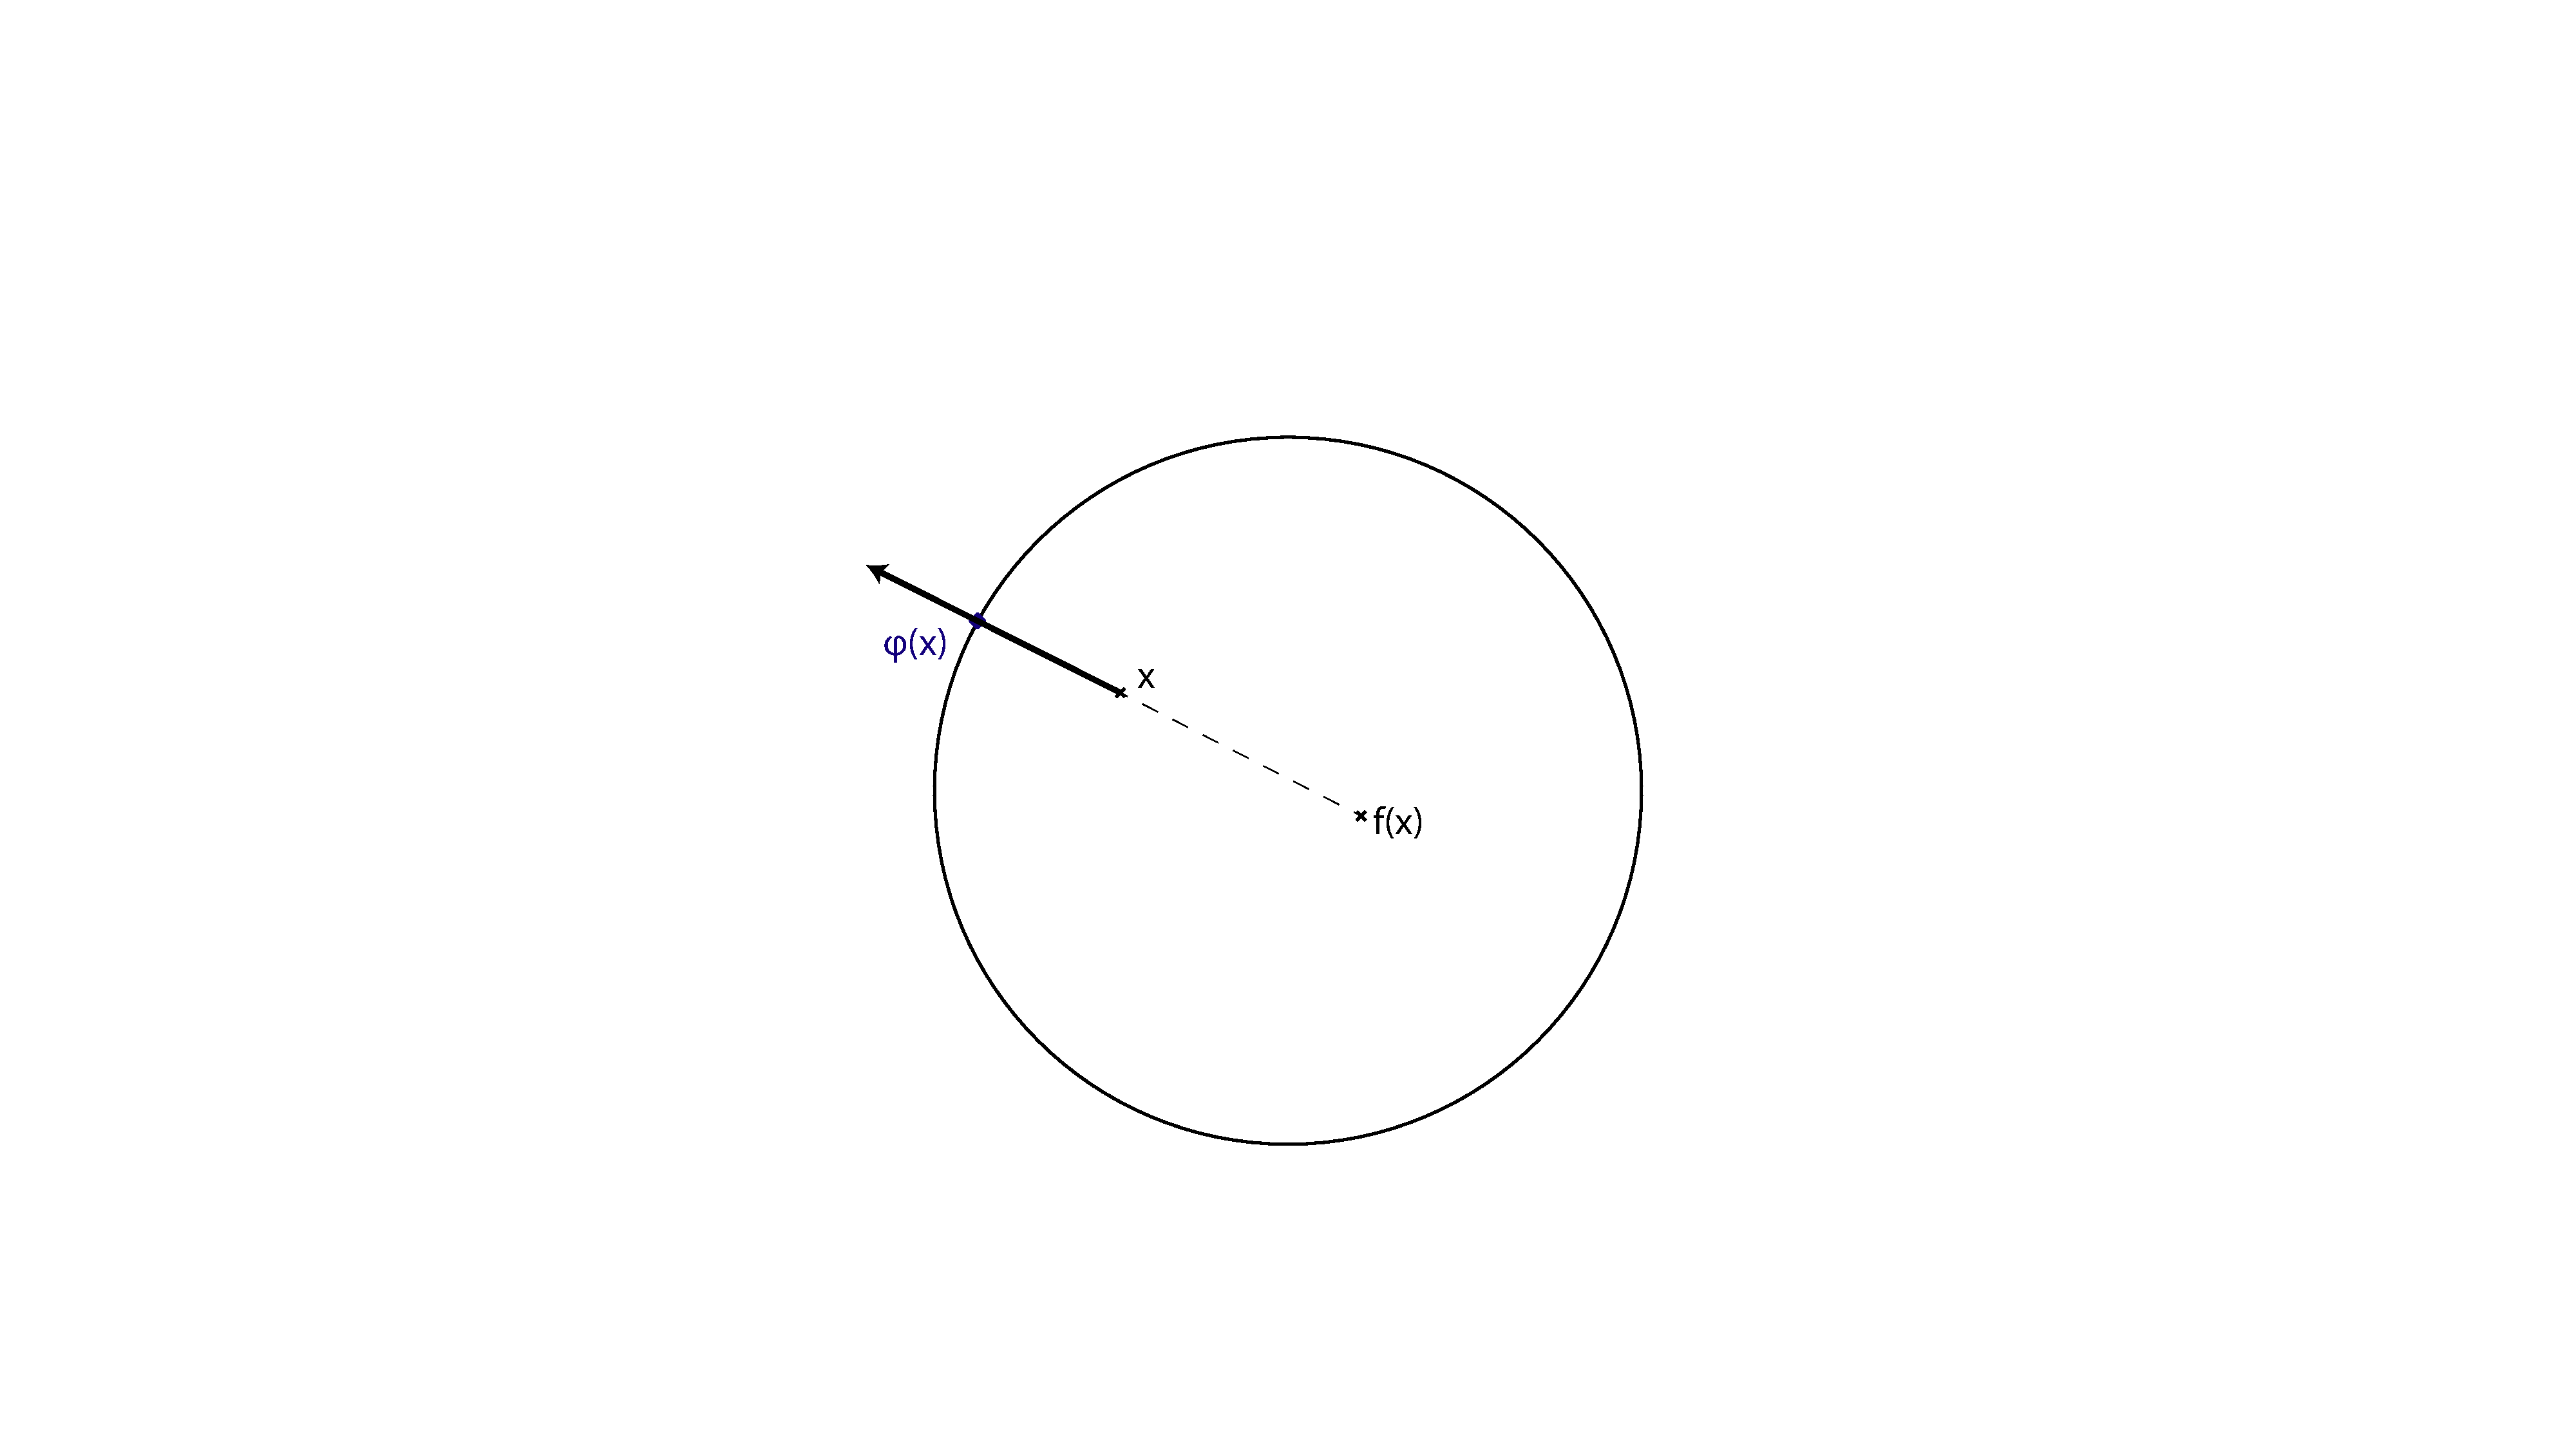
\includegraphics[trim={30em 20em 0 30em},clip,width=1.2\textwidth]{img1.pdf}
	\caption{Définition de $\phi$}
\end{figure}


\subsection{Variantes et applications de Brouwer}


\begin{theoreme}[Point fixe de Schauder] 
	Soit $K$ un convexe fermé sur un Banach. Soit $f \in C ^0\left( K,K \right) $ tel que $\overline{f\left( K \right) }$ est compact . Alors $f$ admet un point fixe.
\end{theoreme}


\begin{proof}
	Prenons $K' := \overline{Hull\left( f\left( K \right)  \right) }$.
	Alors $K'$ est compact (voir \hyperlink{hull}{Prop. 8}).

	De plus, $Hull\left( f(x) \right) \subset Hull\left( H \right) = K$ donc $K' = \overline{Hull\left( f\left( K \right)  \right) } \subset K$ car $K$ fermé. Ainsi $f_{|K'} : K' \to K'$ est continue sur un convexe compact fermé non vide.

	Soit $\varepsilon>0$. Soient $x_1,\ldots, x_I \in K'$ tels que $K' \subset \bigcup_{1\le i\le I} B\left( x_i, \varepsilon \right) $.
	
 On pose $K_{\varepsilon}= Hull\left( \{x_1,\ldots, x_I\}  \right) $ et $		g_{\varepsilon}:  \begin{cases}
		    K' &\longrightarrow K_{\varepsilon} \\
		x &\longmapsto \frac{ \sum_{i=1}^{I} \phi_{i}\left( x \right) x_i}{\sum_{i=1}^{I} \phi_i\left( x \right) }
		\end{cases}$,
	avec 
 
 $\phi_i\left( x \right) := \max\left( 0, \varepsilon - \|x-x_i\| \right) $ (>0 si $x \in  B(x_i, \varepsilon)$).

	Comme $K'\subset \bigcup_{i=1} ^I B\left( x_i, \varepsilon \right) $, or $\sum_{i=1}^{I} \phi_i\left( x \right) >0$ pour tout $x \in K'$ donc $g_{\varepsilon}$ est continue.
 Ainsi $f_{\varepsilon} : \begin{cases}
    K_{\varepsilon} \to  K_{\varepsilon} \\    
    x \mapsto g_{\varepsilon}\left( f\left( x \right)  \right)
 \end{cases}$ est continue. 
 
 De plus, $K_{\varepsilon} \subset  \text{Vect}\left( x_i ~|~1\le i\le I \right) $ est un convexe compact en dimension finie (suffit pour Brouwer).  
 Par le \hyperlink{brouwer}{théorème de Brouwer}, $f_{\varepsilon}$ admet un point fixe $x_{\varepsilon} \in K_{\varepsilon} \subset K'$.
 Par compacité de $K'$, il existe une suite $\left( \varepsilon_{n} \right) _{n\in \mathbb{N}}$ positive, tendant vers $0$ et telle que $x_{\varepsilon_n} \to  x_{*} \in K'$.

	Par ailleurs, pour tout $x \in K'$ \begin{align*}
		\|g_{\varepsilon}\left( x \right) -x\| &\le \frac{\sum_{i=1}^{I} \phi_{i}\left( x \right)\overbrace{\|x-x_i\|}^{\le \varepsilon \text{ si } \phi_{1}\left( x \right) >0}}{\sum_{i=1}^{I} \phi_i\left( x \right) }\\
						       &\le \frac{ \sum_{i=1}^{I} \phi_i\left( x \right) \varepsilon}{\sum_{i=1}^{I} \phi_i\left( x \right) } =\varepsilon
	\end{align*}
	Donc $\|x_{\varepsilon}- f\left( x_{\varepsilon} \right) \| = \| g_{\varepsilon}\left( f\left( x_{\varepsilon} \right)  \right) - f\left( x_{\varepsilon} \right) \| \le \varepsilon$.

	Ainsi $\|x_{*} - f\left( x_* \right) \| \le \limsup \limits_{n\to \infty } \| f\left( x_{ \varepsilon_n} \right) - x_{\varepsilon_n}\| \le \limsup \limits_{n\to \infty} \varepsilon_n = 0$.
\end{proof}

\begin{remarque}
	(Brouwer sur un ensemble autre que $B'\left( 0,1 \right) $)

	\begin{itemize}
		\item  Si $A \subset \mathbb{R}^d $ est homéomorphe à $B'\left( 0,1 \right) $ et $f \in C^0\left( A,A \right) $ alors $f$ a un point fixe.
		\item Si $K \subset \mathbb{R}^d $.
			\begin{itemize}
				\item Soit $x_0 \in K, F = \text{Vect}\{x-x_0 : x \in K\} $
					Alors $K$ est homéomorphe à $F \cap B'\left( 0,1 \right) .$ (Admis)
					Donc $f$ admet un point fixe.
				\item Approche alternative. Soit $P_K$ la projection orthogonale sur $K$.

					Soit $R>0$ tel que $ K \subset B'\left( 0,R \right) .$ Alors $B'\left( 0,R \right) \to  B'\left( 0,R \right) ; x\mapsto f_{\varepsilon}\left( x \right) $ admet un point fixe $x_0 \in B'\left( 0,R \right) $ .

					On a $x_0 = f\left( P_K\left( x_0 \right)  \right) $, donc $x_0 \in K$, donc $x_0 = P_K\left( x_0 \right) $ donc $x_0 = f\left( x_0 \right) $.
			\end{itemize}
	\end{itemize}
\end{remarque}
\begin{remarque}
	Le théorème de Schauder s'étend sur en supposant seulement que $E$ est un espace vectoriel topologique. En particulier, il s'applique aux evtlcs, donc aux topologies faibles.  {\fontencoding{U}\fontfamily{futs}\selectfont\char 49\relax} Il faut que la fonction soit continue par rapport à cette topologie.
\end{remarque}
	
\begin{theoreme}[Cauchy-Arzela-Peano]

	Soit $\Omega \subset \mathbb{R}^d $ ouvert, $x_0 \in  \Omega$.
	Soit $ f \in C^0\left( \R_+^* \times  \Omega, \mathbb{R}^d  \right) $. 
 
        Alors : $\exists  t_0 >0, u \in C^1\left( [0,t_0], \Omega \right),$
        
        $$\begin{cases}
            u'(t) = f(t,u(t)) \forall t \in [0,t_0]\\
            u(0) = x_0
        \end{cases}$$
        
\end{theoreme}
\begin{proof}
	Soit $r_0 >0$ tel que $B'\left( x_0, r_0 \right) \subset \Omega$.
	Soit $t_1 >0$, $C_0 := \sup \{\|f(t,x\| : 0\le t\le t_1, x \in B'\left( x_0, r_0 \right) \} (< \infty$ car $[0,t_1]\times B'(x_0,r_0)$ est compact).
	Soit $t_0 >0$ tel que $C_0 t_0 \le r_0.$

	Posons $K= \mathcal{C}^0([0,t_0], B'( x_0, r_0 ))$. $K$ est un convexe fermé (pour $\| . \|_\infty$).

	Posons $F : \begin{cases}
	    K \to  K \\
            u \mapsto Fu ( t ) := x_0  + \int_{0}^{t} f\left( s,u\left( s \right)  \right) \mathrm{d} s
	\end{cases}$
	\begin{itemize}
		\item $F\left( K \right) \subset K$. En effet, $\|Fu\left( t \right) -x_0\| \le \int_{0}^{t} \underbrace{\|f\left( s,u\left( s \right)  \right) \|}_{\le C_0} \mathrm{d} s \le C_0 t \le C_0t \le r_0$, pour tout $t\in [0, t_0]$.
			De plus, $Fu \in C^1( [0, t_0], B'(x_0,r_0) ) $ en tant que primitive, donc est continue.

		\item $F$ est continue.
			En effet, soit $\omega$ un module d'uniforme continuité de $f$ sur $[0,t_0] \times B'\left( 0,1 \right) $ (on peut se donner un tel module d'uniforme continuité d'après le théorème de Heine).
			Alors pour tous $u,v \in K, \forall t \in [0,t_0] \ $ 
			\begin{align*}
				\left\|Fu\left( t \right) - Fv\left( t \right) \right\| &\le \int_{0}^{t}  \|f(s,u\left( s \right) ) - f\left( s, v\left( s \right)  \right) \|   \mathrm{d} s\\
											&\le \int_{0}^{t} \omega\left( \| u\left( s \right) - v\left( s \right) \| \right) \mathrm{d} s\\
											&\le t_0 \omega\left( \|u-v\|_{\infty} \right) \text{ (on peut toujours supposer $\omega$ croissante)} 
			.\end{align*}

			Donc $\|Fu-Fv\|_{\infty}\le  \omega\left( \|u-v\|_{\infty} \right) $, donc $F$ est uniformément continue et a fortiori, elle est continue.
		\item $\overline{F\left( K \right) }$ est compact.

			En effet, $\forall  u \in K, \forall s \in  [0,t_0], \|Fu\left( t \right) -Fu\left(s \right) \| \le  \left| \int_{s}^{t} \underbrace{\|f\left( x, u\left( x \right)  \right)}_{\le C_0} \| \mathrm{d} x \right| \le C_0 |t-s|$.

			Donc $F \left( K \right) \subset Lip_{C_0}([0,t_0],B'(x_0,r_0))$ qui est compact par le \hyperlink{ascoli}{théorème d'Ascoli}.
   
			Ainsi, $\overline{F\left( K \right) }$ est un fermé dans un compact, donc est compact.

			Par le théorème de Schauder, $F$ admet un point fixe, $ u \in C^0\left( [0,t_0], B'\left( x_0, r_0 \right)  \right) $ telle que $u\left( t \right) = x_0 + \int_{0}^{t} f(s, u\left( t \right) ) \mathrm{d} s $

			Donc $u \in C^1$ et $u' = f\left( s, u\left( t \right)  \right) $.
	\end{itemize}
\end{proof}

\subsection{Stone-Weierstrass}

\begin{theoreme}[Stone-Weierstrass]
	Soit $X$ compact $A \subset C^0\left( X, \mathbb{R} \right) $ algèbre (non forcément unitaire) telle que
	\begin{itemize}
		\item ($A$ sépare les points) $\forall x\neq y \in X, \exists f \in A, f(x) \neq  f(y)$
		\item ($A$ ne s'annule pas simultanément en un point) $\forall x \in X, \exists f \in A, f(x) \neq 0$.
	\end{itemize}

	Alors $\overline{A} = C^0 \left( X,\mathbb{R} \right) $ (norme $\|\cdot \|_{\infty}$ sur $C^0\left(X,\mathbb{R} \right)$ ).
\end{theoreme}

\begin{lemme}
$\overline{A}$ est une algèbre complète unitaire.
\end{lemme}
\begin{proof}
	$\overline{A} \subset C^0\left(X,\mathbb{R}\right)$ est bien une algèbre, et est complète comme fermé d'un complet. 
	Par hypothèse, $\forall x\in X, \exists f_x \in A, f_x\left( x \right) \neq 0 $.
	Posons $V_x := \{y \in X : f_x\left( y \right) \neq 0\} $ qui est ouvert.

	Soit $X = \bigcup_{i=1} ^I V_{x_i}$ une couverture finie de $X$ par compacité, avec $x_1,\ldots,x_I \in X$.

	Alors $f:= \sum_{i=1}^{I} f_i^2 \in A$ et $f>0$ sur $X$.

	Posons $g:= \frac{f}{\|f\|_\infty} \in A$ $0 < g\le 1$ sur $X$.

	Alors $ \mathbf{1} = g \times \frac{1}{g} = g \times \frac{1}{1-(1-g)}  = \sum_{n\in \mathbb{N}}g(1-g)^n$.
En effet, $\|g\left( 1-g \right) ^n\|_{\infty}\le (1-p)^n$ sommable et $g\left( 1-g \right) = \sum_{k=0}^{\infty} \begin{pmatrix} n \\ k \end{pmatrix} (-1)^k g^{k+1} \in A$.

Ainsi, $\mathbf{1} $ est limite uniforme de sommes partielles qui appartiennent à $A$. Dina $\mathbf{1} in \overline{A}$.

\end{proof}

\begin{lemme}
	Soit $ f \in A$ telle que $f\ge 0$ sur $X$ alors $\sqrt{f} \in A$.
\end{lemme}
\begin{proof}
	On pose $g := \frac{f}{\|f\|_\infty}$. On a $g \in A$ et $g \in C^0\left(X,[0,1]\right)  $.
	Soit $0< \varepsilon\le \frac{1}{2}$. Alors $\sqrt{\varepsilon+g} = \underbrace{\sqrt{1 + \left( \varepsilon + g -1 \right) } }_{\in [-1 + \varepsilon, \varepsilon \subset_C  ]-1,1[ }=\sum_{n\in \mathbb{N}} \binom{1/2}{n} \underbrace{ \left( \varepsilon + g -1 \right) ^n}_{\|(\varepsilon+g-1)^n\|\le (1-\varepsilon)^n}$
 
 Et $ \forall n\ge 0, \left( \varepsilon+g-1 \right)^n \in A  $, car $\mathbf{1} \in \overline{A}$.

Avec $\begin{pmatrix} \frac{1}{2}\\ n \end{pmatrix} = \frac{\frac{1}{2} (\frac{1}{2} -1) \ldots (\frac{1}{2} - n+1)}{n!}$.

Par convergence normale de la série, $\sqrt{\varepsilon+g} \in \overline{A}$.

Par ailleurs $\sqrt{g} \le \sqrt{\varepsilon+g}  \le \sqrt{\varepsilon} + \sqrt{g} $.

Donc $\|\sqrt{g} - \sqrt{\varepsilon+g} \|_\infty \le \sqrt{\varepsilon} $ donc $\sqrt{g} \in \overline{A}$ par complétude de $\overline{A}$.
\end{proof}

\begin{corollaire}
	Soit $f \in A$ alors $|f| = \sqrt{f^2}  \in \overline{A}$.

	Soient $f,g \in A$, alors $\max\left( f,g \right), \min\left( f,g \right) \in \overline{A}$

	Si $1\ge f\ge 0$ sur $X$, alors  
 $$\frac{1}{f} = \frac{1}{1-(1-f)}= \sum_{n\in \mathbb{N}} (1-f)^n \in \overline{A}$$
\end{corollaire}
\begin{lemme}
	Soient $V\subset X$ ouvert et $x \in V$.
	Alors $\exists f \in \overline{A}$, $0\le f\le 1$, $f(x)=1, f(y) = 0, \forall y \not\in V$.
\end{lemme}
\begin{proof}
Soit $y\neq x$. alors $\exists  f_y \in A$, $f_y\left( x \right) \neq  f_{y}\left( u \right)$

On choisit $\alpha,\beta \in \mathbb{R}$ tels que $g_{y} := \alpha f + \beta $ satisfaisant $g_{y}\left( x \right) =1, g_{y}\left( y \right)=-1$.
On pose $V_g= \{z \in X : f_{y\left( z \right) <0}\} $, ouvert contenant $y$.

Par compacité on dispose de $y_1,\ldots,y_I \in X$ tels que $X = V \cup \bigcup_{i=1} ^I V_{y_i}$. Puis $g\left( z \right)  := \max\left( 0, \min\left( 1, \min \limits_{1\le i\le I} g_{y_i}\left( z \right)  \right)  \right) \in \overline{A}$ convient.
\end{proof}
\epigraph{\textit "On a assez de lemmes pour avancer"}{Jean-Marie Mirebeau}

\begin{proof}
	(Stone-Weierstrass)

	Soit $f \in C^0\left(X,\mathbb{R}\right)  $ que l'on souhaite approcher. Quitte à considérer $\alpha f + \beta$, avec $\alpha\neq 0, \beta \in \mathbb{R}$ on peut supposer $ 0\le f\le 1$ sur $X$.

	Soit $\varepsilon > 0$.

	$\forall x \in X$, soit $V_x = \{{y \in X : |f\left( x \right) -f\left( y \right) | \le \varepsilon}\} $.

	Par compacité, $\exists x_1,\ldots, x_I \in X, X = \bigcup_{i=1} ^I V_{x_i}$.

Soit $y \in X$ arbitraire. Soit $1\le i\le I$ tel que $y \in V_{x_i}$. Soit $\phi_{y} \in \overline{A}, 0\le \phi_y\le 1$ tel que $\phi_{y} \left( y \right) =1$ et $\text{supp} \phi_y \subset V_{x_i}$.

Posons $W_y := \{z \in X : \phi_y\left( z \right) > 1- \varepsilon\} $, par compacité $\exists y_1,\ldots,y_J$ tel que $X = \bigcup_{i=1} ^J W_{y_j}$.

Posons $g\left( x \right) := \max \limits_{1\le j\le J} \phi_{y_j}\left( x \right) f\left( y_j \right) $.

\begin{itemize}
	\item On a $g\left( x \right) \le f\left( x \right) + 2 \varepsilon$

		En effet, si $\phi_{y_j}\left( x \right) \neq 0,$ alors $x,y_j \in V_{x_i}$, pour un certain $1\le i\le I$.

		Donc $\phi_{y_j} f\left( y_j \right) \le f\left( y_j \right) \le f\left( x \right) + | f\left( x \right) - f(x_i)| + |f\left( x_i \right) - f\left( y_j \right) |$.
	\item On a $f\left( x \right) \le g\left( x \right) + 3 \varepsilon$.

		En effet, soit $y_j$ telle que $x \in W_{y_j}$. Soit $1\le i\le I$ tel que $W_{y_j} \subset V_{x_i}$.

		Alors 
		\begin{align*}
		g\left( x \right) &\ge \phi_{y_j}\left( x \right) \\
				  &\ge f\left( y_j \right) \\
				  &\ge (1-\varepsilon) \left( f(x)- \underbrace{|f\left( x \right) - f\left( x_i \right) |}_{\le  \varepsilon} - \underbrace{|f\left( x_i \right) - f\left( y_j \right) |}_{\le \varepsilon} \right)
				  \\
      &\ge \left( 1-\varepsilon \right) \left( f\left( x \right) - 2 \varepsilon \right)
				  \ge f\left( x \right) - 3 \varepsilon.
			  .\end{align*} 
			  D'où le résultat.
\end{itemize}
\end{proof}

\begin{corollaire}
	Soit $X\subset \mathbb{R}^d $ compact alors $\mathbb{R}[X_1,\ldots,X_d]$ est dense dans $C^0\left(X,\mathbb{R}\right)  $ pour la norme $\|\cdot \|_\infty$.
\end{corollaire}

\begin{corollaire}
	(Stone-Weierstrass complexe)
	Soit $X$ compact $A \subset C^0\left(X,\mathbb{C} \right)  $ une algèbre qui 
	\begin{itemize}
		\item (sépare les points) $\forall x \neq y \in X \exists f \in A, f(x) \neq f(y)$
		\item (ne s'annule pas pas simultanément en un point) $\forall x \in X \exists f \in A f\left( x \right) \neq 0$.
		\item (stabilité par conjugaison) $\forall f \in A, \overline{f} \in A $
	\end{itemize}
	Alors $\overline{A} = C^0\left(X,\mathbb{C} \right)  $.
\end{corollaire}

\begin{proof}
	Si $f \in A$ alors $\Re\left( f \right) := \frac{f+\overline{f}}{2}$ et $\Im \left( f \right) = \frac{f-\overline{f}}{2}$ sont dans $A$. Donc $A \cap C^0\left(X,\mathbb{R}\right)  $ satisfait les hypothèses de Stone Weierstrass réel. 

	Donc $\overline{A \cap C^0\left(X,\mathbb{R}\right)  } = C^0\left(X,\mathbb{R}\right)  $.

	Si $f \in C^0\left(X,\mathbb{C} \right), \varepsilon>0 $ alors $\exists  g,h \in A \cap  C^0\left(X,\mathbb{R}\right) \| \Re\left( f \right) -g\|_\infty\le \varepsilon $ et $\| \Im\left( f \right) - h\|_{\infty}\le \varepsilon$. Donc $\|f - (g+ih)\|_\infty\le 2 \varepsilon.$

	D'où la densité.
\end{proof}

\begin{corollaire}
	Soit $X \subset \mathbb{C} ^d$ compact.
	Alors $\mathbb{C} [X_1, \overline{X_1},\ldots, X_d, \overline{X_d}]$ est dense dans $C^0\left(X,\mathbb{C} \right)  $.
\end{corollaire}
\begin{remarque}
	Soit $B = B_{\mathbb{C} }'\left( 0,1 \right), f \in C^0\left(B,\mathbb{C} \right)  $.
	Sont équivalents : 
	\begin{enumerate}
		\item $f \in \overline{\mathbb{C} [X]}$
		\item $f$ est développable en série entière de rayon de convergence $1$.
		\item $\forall z \in B\left( 0,1 \right) $, $f\left( z \right) = \frac{1}{2i  \pi}\int_{0}^{\pi} \frac{f\left( \text{e}^{it} \right)  i\text{e}^{it}}{\text{e}^{it} -z} \mathrm{d} t$
	\end{enumerate}
\end{remarque}

\begin{proof} Montrons $2 \Rightarrow 1 \Rightarrow 3 \Rightarrow 1$ :


\underline{$2\Rightarrow 1$} : On commence par définir pour tout $\varepsilon > 0 $ la fonction $f_\varepsilon(z) = f((1-\varepsilon)z)$.

On remarque que $f_\varepsilon \xrightarrow[\varepsilon \to 0]{} f $ uniformément (car $f \in \mathcal{C}^0(B,\mathbb{C})$ est uniformément continue).
De plus, la série entière de $f$ converge uniformément sur $B(0,1-\varepsilon) \subset_C B$. Ainsi, 

$$\forall z \in B, f_\varepsilon(z) = \lim_{n \to +\infty} \underbrace{\sum_{k=0}^n a_k(1-\varepsilon)^k z^k}_{\in \mathbb{C}[X]} \text{ uniformément}$$

Donc $f_\varepsilon \in \overline{\mathbb{C}[X]}$, et 
$$f \in \overline{\mathbb{C}[X]}$$
 
\underline{$1\Rightarrow 3$} :

Soient $z \in \mathbb{C}$ tel que $|z|<1$ et $P = \sum_{k=0}^n a_k X^k \in \mathbb{C}[X]$, on a :
 
\newcommand\eit{\text{e}^{it}}
	\begin{align*}
		\int_{0}^{2\pi} \frac{P\left( \text{e}^{it} \right) i \text{e}^{it}}{\text{e}^{-it} -z} \mathrm{d} t &= i \int_{0}^{2\pi} \frac{P\left( \eit \right) }{1 - z \eit} \dd t  \\
		&= i \int_{0}^{2 \pi} P\left( \eit \right) \sum_{n = 0}^{+\infty} \text{e}^{-int} z^n \mathrm{d} t   \\
		&= i \sum_{n=0}^{+\infty} z^n \underbrace{\int_{0}^{2 \pi} P\left(  \eit \right) \text{e}^{-int} \mathrm{d} t}_{=2\pi a_n}   \\
		&= 2 i \pi \sum_{k=0}^{n} a_k z^k = 2 i \pi P\left( z \right)  \\
	\end{align*}

Puis sachant que $f \in \overline{\mathbb{C}[X]}$, par une intervertion de limite-intégrale, on obtient bien l'égalité souhaitée : 

$\underline{3\Rightarrow 2}$ :
	Soit $|z| <1$. On pose  pour tout $n \in \mathbb{N}$, $a_n = \frac{1}{2\pi}\int_0^{2 \pi} f(e^{it})e^{-int}\mathrm{d}t$.

On a :

\begin{align*}
    f(z) &= \frac{1}{2i\pi} \int_0^{2\pi} \frac{f(e^{it}ie^{it}}{e^{it}-z} \mathrm{d}t\\
    &= \frac{1}{2\pi}\int_0^{2\pi} f(e^{it}) \frac{1}{1-ze^{-it}} \mathrm{d}t \\
    &= \frac{1}{2\pi}\int_0^{2\pi} f(e^{it})\sum_{n=0}^{+\infty}e^{-int}z^n \mathrm{d}t \\
    &\underset{(*)}{=} \sum_{n=0}^{+\infty} \frac{1}{2\pi} \int_{0}^{2\pi} f(e^{it}) e^{-int} z^n \mathrm{d}t \\
    &= \sum_{n=0}^{+\infty} a_n z^n
\end{align*}

$(*)$ : On peut intervertir car $f \in \mathcal{C}^0(B,\mathbb{C})$, et $|z| < 1$.

Par les trois points précédents, on obtient bien l'équivalence souhaitée.

\end{proof}


\subsection{Opérateurs linéaires compacts}
\begin{definition}
    Soit $E,F$ evn, $T\in L(E,F)$. On dit que $T$ est compact ssi $\overline{T(B_E(0,1)}$ est compact. On note $L_C(E,F)$ l'ensemble des opérateurs compacts.
\end{definition}

\begin{remarque}
    Si $T\in L_C(E,F)$, alors $dim[\underbrace{\ker(Id-T)}_{\mathclap{E_1}}]<\infty $. En effet $\forall x\in B'_{E_1}(0,1),\ (Id-T)x=0, $ donc $Tx=x$ donc $\underbrace{T(B'_{E_1}(0,1))}_{\mathclap{\subset \overline{T(B_E(0,1))}\text{ compact}}}=B'_{E_1}(0,1).$ \\
    Ainsi $B'_{E_1}(0,1)$ est un fermé donc compact donc $dim(E)<\infty $ par le théorème de Riesz.
\end{remarque}
\begin{theoreme}[Alternative de Fredholm]
    Soit $E$ un Banach, $T\in L_C(E,F)$ tq $\ker(Id-T)=\{0\} .$ Alors $Im(Id-T)=E,$ et $Id-T$ a un inverse continu.
\end{theoreme}
\begin{proof}
    Montrons d'abord que $\underbrace{Im(Id-T)}_{(Id-T)E}$ est fermé.\\
    Soit $(u_n)$ une suite convergente à valeurs dans $(Id-T)$. $u_n=v_n-Tv_n$, $u_n\to u_*.$ Supposons par l'absurde que $\|v_n\|\to \infty .$ Posons $w_n=\frac{v_n}{\|v_n\|}.$ Alors $v_n=u_n+Tv_n.$ Donc $w_n=\underbrace{\frac{u_n}{\|v_n\|}}_{\substack{\to 0,\text{ car}\\u_n\text{ bornée}}}+\underbrace{Tw_n}_{\substack{\text{à valeur dans}\\\text{$\overline{T(B'_E(0,1))}$ compact}}}$.\\
    $\exists \varphi  $ extractrice, telle que $Tw_{\varphi (n)}$ converge, $Tw_{\varphi (n)}\to w_*,$ ie $w_{\varphi (n)}=\frac{u_{\varphi (n)}}{\|v_{\varphi (n)}\|}+Tw_{\varphi (n)}\to w_*.$ Donc on a
     $\left\{\begin{aligned}
             Tw_{\varphi (n)}&\to w_*\hspace{0.9em} \text{par compacité}\\
             w_{\varphi (n)}&\to w_* \hspace{0.9em} \text{par l'argument précédent}\\
         Tw_{\varphi (n)} &\to Tw_* \ \text{par continuité}
    \end{aligned}\right.$.
Donc $Tw_*=w_*$ par unicité de la limite, et de plus $\|w_*\|=\lim\limits_{n \to \infty} \|w_n\|=1.$ Ainsi $w_*\in \ker(Id-T)=\{0\} ,$ contradiction! On a donc $v_n$ bornée et $\exists \psi$ extractrice tq $Tv_{\psi(n)}$ converge. Alors par le même raisonnement $v_{\psi(n)}=\underbrace{u_{\psi(n)}}_{\text{cv}}+\underbrace{Tv_{\psi(n)}}_{\text{cv}}$, donc $\underbrace{u_{\psi(n)}}_{\to u_*}=\underbrace{v_{\psi(n)}}_{\to v_*}-\underbrace{Tv_{\psi(n)}}_{Tv_*}.$ Donc $u_*=v_*-Tv_*\in (Id-T)E$ d'où la fermeture de $(Id-T)E$.\\
Montrons maintenant que $(Id-T)E=E.$ Posons $F_n=\left( Id-T \right) ^nE,\forall n\ge 0. $ Par la première partie, $F_1\subset F_0$ et fermé. Donc c'est un Banach stable par $T$ donc $T\in L_C(F_1)$ par la première partie. $F_2$ est fermé et par récurrence $F_n$ est fermé pour tout $n\ge 0.$ Si par l'absurde, $\underbrace{F_0\backslash F_1}_{E\backslash [(Id-T)E]}\neq \emptyset ,$ choisissons $x_0\in F_0\backslash F_1$. Alors $x_n:=T^nx_0\in F_n\backslash F_{n+1}$ par injectivité de $Id-T.$ [En effet si on avait $x_n\in F_{n+1},$ $\left( Id-T \right) ^nx_0=x_n=\left( Id-T \right) ^{n+1}x_0$ donc $x_0=(Id-T)y\in F_1,$ impossible]. Ainsi $F_{n+1}\not\subset F_n.$ Par le lemme de Riesz, on peut choisir $y_n\in F_n$ tq $\|y_n\|=1$ et $d(y_n,F_{n+1})\ge \frac{1}{2}.$ Pour $m<n$ on a : $Ty_m-Ty_n =y_m+\underbrace{\underbrace{(T-Id)y_m}_{\in F_{m+1}}-\underbrace{Ty_n}_{\in F_n}}_{\in F_{m+1}}$. Donc $\|Ty_m-Ty_n\|\ge d(y_m,F_{m+1})\ge \frac{1}{2}.$ Donc $(Ty_n)$ n'a pas de sous suites convergente, ce qui contredit la compacité de $\overline{T(B(0,1))},$ puisque $\|y_n\|=1.$  \\
On a montré que $(Id-T)E=E.$ Ainsi $Id-T$ est injective et surjective donc bijective. Par le théorème de Banach, les bijection linéaires continues dans un Banach sont d'inverse continue.
\end{proof}
\begin{lemme}
    Soit $K\in C^0([0,1],\mathbb{R} ),$ posons $\forall f\in C^0([0,1],\mathbb{R} ),\ \mathcal{K}(f)(x):=\int_0^1K(x,y)f(y)dy$. C'est un opérateur compact de  $(C^0([0,1],\mathbb{R} ),\|.\|_\infty )$.
\end{lemme}
\begin{proof}
    Soit $w$ un module de continuité de $K,$ alors $\forall f\in C^0([0,1],\mathbb{R} ),\ \forall x,y\in [0,1], $,
    \begin{align*}
        |\mathcal{K}(f)(x)| &\le \int_{0}^{1} K|K(x,y)| |f(y)| dy \\
        &\le \|K\|_\infty \|f\|_\infty \\
        |\mathcal{K}(f)(x)-\mathcal{K}(f)(y)| &= |\int_{0}^{1} K(x,z)f(z)dz-\int_{0}^{1} K(x,z)f(z)dz  | \\
                                              &\le \int_{0}^{1} |\underbrace{K(x,z)-K(y,z)}_{\le w(|x-y| }||f(z)| dz\\
                                              &\le w(|x-y| )\|f\|_\infty
    .\end{align*}

    Ainsi $\{\mathcal{K}(f)\ |\ f\in C^0([0,1]),\ \|f\|_\infty \le 1\} $ est uniformément borné et équipotente, donc est relativement compact par le théorème d'alcali. Ainsi $\mathcal{K}$ est un opérateur compact.
\end{proof}
\begin{corollaire}
    Soit $K\in C^0([0,1]^2,\mathbb{R}_+ ),$ $g\in C^0([0,1])$ et $K(x,y)=K(y,x)\forall x,y.  $  Alors $\exists !f\in C^0([0,1]),\ \forall x,\ \int_{0}^{1} K(x,y)\left( f(y)-f(x) \right) dy-f(x)=g(x).  $
\end{corollaire}
\begin{proof}
    Posons $k(x)=\int_{0}^{1} K(x,y)dy .$ L'équation complétée correspond à $\mathcal{K}(f)(x)-(1+k(x))f(x)=g(x).$ C'est à dire $\hat{\mathcal{K}}(f)-f=\hat{g},$ avec $\hat{\mathcal{K}}=(\underbrace{\left( 1+k \right) ^{-1} }_{\text{op compact}}\underbrace{\mathcal{K}}_{\text{op compact}}.$ Donc $\hat{\mathcal{K}}$ est compact comme composée d'un opérateur compact et d'un opérateur continue. Par l'alternative de Fredholm, il suffit de montrer que $\ker(\hat{\mathcal{K}}-Id)=\{0\} .$ Par l'absurde, soit $f\in C^0([0,1])$ tq $\hat{\mathcal{K}}(f)=f,$ ie $\mathcal{K}(f)=(1+k)f.$ \\
    Donc $\underbrace{\int_{x=0}^{1} \int_{y=0}^{1} K(x,y)\left( f(y)-f(x) \right) dy \cdot f(x)dx}_{=-\frac{1}{2}\int_{0}^{1} \int_{0}^{1} K(x,y)\left( f(x-f(y) \right) ^2dydx \text{ par sym de }K } =\int_0^1 f(x)^2dx $.\\
    Finalement, $\int f^2\le 0$ donc $f=0$ d'ou l'injectivité.
\end{proof}
\begin{definition}
    Soit $E$ un evn, $T\in L(E,F),$ le spectre de $T$ est $\sigma(T):=\{\lambda\in \mathbb{K}\ |\ \lambda Id-T \text{ n'a pas d'inverse continue}\} $.
\end{definition}
\begin{propriete}
    Soit $E$ un Banach, $T\in L(E,F).$
    \begin{enumerate}[label=(\roman*)]
        \item Si $dim(E)=\infty $ alors $0\in \sigma(T)$
        \item $\forall \lambda\in \sigma(T)\backslash \{0\}, \exists x\in E,\ Tx=\lambda x. $
        \item $\forall \lambda \in  \sigma(T)\backslash \{0\} ,\ \exists m=m(\lambda),\ \ker(\left( \lambda -T \right) ^m)=\ker\left( (\lambda-T)^{m+1} \right)  $. De plus, $\ker\left( (I-T)^m \right) $ est de dimension finie
        \item L'ensemble $\sigma(T)$ est dénombrable, et $0$ est le seul point d'accumulation possible.
    \end{enumerate}

\end{propriete}
\begin{proof}
    \begin{enumerate}[label=(\roman*)]
        \item Si $0\not\in \sigma(T),$ alors $T^{-1} $ existe et est continue. Donc \\
            $\underbrace{T^{-1} (\overline{T(B(0,1))})}_{\substack{\text{compact comme image}\\ \text{d'un compact par }T^{-1} \text{ $c^0$}}}\supset \underbrace{B'(0,1)}_{\text{fermé}}$. Donc $B'(0,1)$ est compact, donc $dim(E)<\infty $ par le théorème de Riesz.
        \item Application de l'alternative de Fredholm à $T.$
        \item Posons $F_n\subsetneq F_{n+1}$, en choisissant $x_n\in F_n$ tq $\|x_n\|=1$ et $d(x_n,F_{n+1)\ge \frac{1}{2}}.$\\
            Soit $m<n$ $Tx_m-Tx_n=\underbrace{\lambda x_m}_{\in F_m} + \underbrace{(T-\lambda)x_m}_{\in F_{m+1}}-\underbrace{\lambda x_n}_{\in F_n}-\underbrace{(T-\lambda)x_n}_{\in F_{n+1}}. $  Donc $\|Tx_m-Tx_n\|\ge d(\lambda x_m,F_{m+1})\ge \frac{|\lambda |}{2}. $ Donc $(Tx_n)$ n'a pas de sous suite convergente, contredit la compacité de $T.$ Donc $\exists m,\ \ker\left( (\lambda-T)^m \right) =\ker\left( (\lambda-T)^{m+1} \right) $ comme annoncé.\\
            De plus, $D_\lambda=\ker\left( (\lambda-T)^m \right) $ est stable par $T,$ et $\forall \times \in E_\lambda,\ (\lambda-T)^mx=0, $ donc $\lambda^mx=\underbrace{\sum\limits_{k=0}^{m-1} \left( -1 \right) ^k\lambda^kT^{m-k}x}_{TQ(T)x}$. Donc $B_{E_\lambda}(0,|\lambda| ^m)=\underbrace{\underbrace{TQ(T)}_{\text{op compact}}B_{E_\lambda}(0,|\lambda| ^m}_{\text{d'adhérence compact}}$. Donc $B'_{E_\lambda}(0,|\lambda|^m)$ est compact et $dim(E_\lambda)<\infty .$
        \item Supposons que $\sigma(T)$ a un point d'accumulation $\lambda x\neq 0.$ Alors on a $\lambda m\to \lambda x$ avec $\lambda m\neq \lambda x.$ On choisit $x_n\neq 0,\ Tx_n=\lambda _x x_n$. On pose $F_n=\{x_1,\cdots,x_n\} ,$ on choisit $y_n\in F_n$ tq $\|y_n\|=1$ et $d(y_n,F_{n+1})\ge \frac{1}{2}.$ par lemme de Riesz. Comme avant on se ramène à $(Ty_n)$ qui n'a pas de sous suite convergente ce qui est contradictoire. \\
            Par ailleurs, $\sigma(T)\subset B'(0, \vertiii{T})$ pour tout opérateur continue puisque $\left( \lambda I-T \right) ^{-1} =\frac{1}{\lambda}\left( I-T x \right) ^{-1} =\frac{1}{\lambda}\sum\limits_{n\ge 0}^{} \left( \frac{T}{\lambda} \right) ^n$ si $|\lambda| \ge \vertiii{T}$. Ainsi pour tout $\varepsilon >0,$ $\sigma(T)\backslash B_\mathbb{K}(0,\varepsilon )$ est un ensemble borné sans point d'accumulation, donc fini. Donc $\sigma(T)\backslash \{0\} =\bigcup\limits_{n\ge 1} \sigma(T)\backslash B(0,\frac{1}{n})$ est dénombrable.
    \end{enumerate}
\end{proof}

\begin{definition}[Propriété d'approximation]
    Un evn $E$ a la PA si\\
    $\forall \varepsilon >0,\ \forall K\subset _CE,\ \exists T\in L_f(E,):=\{T\in L(E)\ |\ dim(Im(T))<\infty \} , $ tel que $\forall x\in K,\ \|Tx-x\|\le \varepsilon  $
\end{definition}
\begin{ex}
    Tout espace de Hilbert à la PA. En effet, soit $x_1,\cdots, x_I\in K$ tels que $K\subset \bigcup\limits_{1\le i\le I}B(x_i,\varepsilon ).$ Soit $T$ la projection orthogonale sur $Vect(x_1,\cdots,x_I).$ Alors $T$ est linéaire, continue et $\forall x\in K,\ \|Tx-x\|=\min_{1\le i\le I}\|x_i-x\|\le \varepsilon  $ \\
    On sait que $L^p(X,\mu)$ pour tout $1\le p\le \infty $ a la PA. \'Egalement,$C^0_b(X)$ a la PA pour tout espace métrique $(X,d).$
\end{ex}
\begin{propriete}
    Soit $E$ un evn et $F$ un espace de Banach. Alors $L_c(E,F)$ est fermé et $L_c(E,F)\supset \overline{L_f(E,F)}$ avec égalité si $F$ a la PA. \\
    De plus, si $T\in \bar{L_f(E,F)}$, alors $T:\left( B'_E(0,1), \text{faible} \right) \to (F,\|.\|_F)$ est continue.
\end{propriete}
\begin{proof}
    \begin{itemize}
        \item Fermeture de $L_c(E,F)$. Soit $T\in \overline{L_c(E,F)}, \varepsilon >0$. Soit $T_0\in L_c(E,F)$ tq $\|T-T_0\|\le \varepsilon .$ Comme $K_0=\overline{T_0(B)}$ est compact (avec $B=B_E(0,1)$), il existe $x_1,\cdots,x_n\in K_0$ tq $K_0\subset \bigcup\limits_{i\le  I}B(x_i,\varepsilon ).$ Alors $K=\overline{T(B)}\subset \bigcup\limits_{1\le i\le I} B(x_i,2\varepsilon )$. Ainsi $K$ est un précomact, et un complet car fermé dans $F$ Banach, donc compact.
    \item Les opérateurs de rand fini sont compacts. En effet, si $T\in L_f(E,F),$ alors $\overline{T(B)}\subset \underbrace{Im(T)\cap B'_F(0, \vertiii{T})}_{\substack{\text{fermé borné en dim finie}\\\text{donc compact}}}$. Donc $T(B)$ est une partie fermée d'un compact donc compact. Ainsi $L_f(E,F)\subset L_c(E,F)$ fermé et $\overline{L_f(E,F)}\subset L_c(E,F)$.
    \item Montrons que $L_c(E,F)=\overline{L_f(E,F)}$ si $F$ a la PA. Soit $T\in L_c(E,F),\varepsilon >0.$ Soit $K=\overline{T(B)}$, soit $P\in L_f(F)$ tq $\|Py -y\|\le \varepsilon ,\forall y\in K.  $. Alors $P\circ T$ est de rang fini et $\sup_{x\in B}\|P(Tx)-Tx\|=\vertiii{P\circ T-T}\le \varepsilon $ , donc $T\in L_f(E,F).$
    \item Continuité faible $\to $ forte. Soit $T\in L_f(E,F),$ soit $f_1,\cdots,f_n$ une base de $Im(T).$ On écrit $T(x)=\sum\limits_{1\le i\le n}^{} f_il_i(T(x))\le \sum\limits_{i=1}^{n} \|f_i\||\underbrace{l_i(T(x))}_{\mathclap{\substack{l_i\circ T\in E^*\\\text{la $i_{\text{eme}}$ coordonnée}}}}| $ Donc $T:\left( E,\left( | \varphi (x)|  \right) _{\varphi \in E^*} \right) \to \left( F,\|.\|_F \right) $ est continue. Soit $T\in \overline{L_f(E,F)}$ et $T_n\in L_f(E,F)$ tq $\vertiii{T-T_n}\to 0.$ Alors $T_n$ est continue pour la topologie faible et converge uniformément vers $T$ donc $T$ est continue.
    \end{itemize}
\end{proof}
